\documentclass[pageno]{jpaper}

%replace XXX with the submission number you are given from the ASPLOS submission site.
\newcommand{\asplossubmissionnumber}{329}

\usepackage{mathptmx} % This is Times font
\usepackage[table]{xcolor} % xcdraw causes compilation error
%\usepackage{amssymb}
\usepackage{pifont}

\newcommand{\cmark}{{\color{green}\ding{51}}}%
\newcommand{\xmark}{{\color{red}\ding{55}}}%

\usepackage{fancyhdr}
\usepackage[normalem]{ulem}
%\usepackage[hyphens]{url}
\usepackage[sort,nocompress]{cite}
%\usepackage[final]{microtype}
\usepackage{flushend}
\usepackage{subfig}
\usepackage{graphicx}
\usepackage{tikz}
\usepackage{algorithm}
\usepackage[noend]{algpseudocode}

\def\UrlBreaks{\do\/\do-\do_}
\usepackage[hyphenbreaks]{breakurl}
\usepackage{hyperref}
%\usepackage{comment}

% Always include hyperref last
%\usepackage[bookmarks=true,breaklinks=true,letterpaper=true,colorlinks,linkcolor=black,citecolor=blue,urlcolor=black]{hyperref}

\newcommand\javier[1]{\noindent{\color{cyan} {\bf \fbox{Javier}} {\it#1}}}
\newcommand\abhishek[1]{\noindent{\color{green} {\bf \fbox{Abhishek}} {\it#1}}}
\newcommand\babak[1]{\noindent{\color{magenta} {\bf \fbox{Babak}} {\it#1}}}
\newcommand\djordje[1]{\noindent{\color{purple} {\bf \fbox{Djordje}} {\it#1}}}
\newcommand\chart[1]{\noindent{\color{cyan} {\bf \fbox{Chart}} {\it#1}}}



\usepackage{booktabs}
\usepackage{multirow}

\sloppy



\newcommand*\circled[1]{\tikz[baseline=(char.base)]{
            \node[shape=circle,draw,inner sep=0.5pt] (char) {#1};}}

\begin{document}

%\title{
%Instructions for Submission to ASPLOS 2018}

\title{Set-Associative Virtual Memory Regions}

\date{}
\maketitle

\thispagestyle{empty}

\begin{abstract}

As the computing industry embraces increasingly large and heterogeous systems, 
a key research challenge is the question of how to integrate hardware accelerators in
modern platforms without impacting the conventional virtual memory (VM)
abstractions modern complex software stacks rely on. Unfortunately, VM
support for accelerators is fundamentally different from CPU's due to
prohibitive TLB reach requirements, tight area and power budgets, and increasing
latency of page table walks. Moreover, recent proposals for
accelerator VM break conventional VM abstractions with intrusive OS
changes to facilitate address translation.


We propose SpryVM, a set-associative VM architecture for large heterogeneos systems.
We show that maintaining the portion of the address space accelerators operate
on set-associatively has virtually no impact on page fault traffic, but 
significantly reduces translation hardware requirements and page-walk latency. 
A tiny reduction in the associativity of virtual-to-physical address mapping allows 
SpryVM to partition the memory space and delegate the address translation to the
memory partition that holds the data, where memory-side per-partition TLBs and MMUs
can locally translate addresses at lower latency and with higher efficiency. In doing so, SpryVM 
significantly improves TLB hit rates and breaks page walk-data fetch serialization upon
TLB misses. SpryVM achieves within 1.2\% and 0.6\% of ideal translation in scenarios 
where working sets are memory-resident and exceed the available memory capacity,
respectively. Finally, we implement spryVM in stock Linux, showing
that these benefits are achievable while retaining conventional VM
abstractions and with only modest changes to existing VM software
stacks.



\end{abstract}


\section{Introduction}
\label{sec:intro}
As the computing industry embraces hardware specialization, research
questions pertaining to the system integration of accelerators in
modern platforms are becoming increasingly important. One such
question is that of how to expose the virtual memory (VM) abstraction
to accelerators. While initial solutions allow accelerators to have
direct physical access to memory, the consequent lack of protection,
isolation and paging significantly complicates the software
stack. More recent studies have argued that the conventional VM
abstraction and a global address space programming model is best for
software development enabling "a pointer is a pointer everywhere"
semantics~\cite{pichai:architectural, power:supporting,
  haria:devirtualizing, vesely:observation, ausavarungnirun:mosaic},
extending memory protection to accelerators, and obviating the need
for manual inter-CPU-accelerator data marshalling.

Unfortunately, it is challenging to extend conventional VM to
accelerators in an efficient manner. While general-purpose cores rely
on large hiearchical TLBs to implement VM
efficiently, such large structures are ill-suited to area-constrained 
accelerators. This is true for a wide spectrum of
accelerators ranging from programmable GPGPUs
\cite{pichai:architectural, power:supporting} to graph processing
hardware \cite{haria:devirtualizing} to even more area-contrained
processing in/close-to memory techniques \cite{picorel:near-memory}.

In response, several recent studies propose changes to conventional
TLB hardware and the memory allocation/management stack for efficient
address translation and page management on accelerators
\cite{pichai:architectural, power:supporting,
  ausavarungnirun:mosaic}. Among the most promising are techniques
that obviate the need for large TLBs by relying on the concept of
translation contiguity, situations where large contiguous 
ranges of virtual pages are mapped to a corresponding range
of spatially-adjacent physical pages. The idea is that TLBs would
compress or coalesce these ranges of translations into a single
hardware entry, greatly reducing address translation pressure. While
some of these techniques rely on translation contiguity that OSes may
serendipitously generate \cite{pham:colt, bhattacharjee:large-reach, 
cox:efficient, pham:increasing}, the most successful ones are those that
rely on changes to the OS's memory allocation path so that it produces
vast swaths of translation contiguity
\cite{haria:devirtualizing}. Unfortunately, these techniques (and
similar ones proposed for CPUs \cite{basu:efficient, gandhi:range})
sacrifice OS flexibility to generate translation contiguity by
requiring, for example, identity mapping (which can be difficult to
achieve in real-world cloud settings where many applications utilize a
machine), or at-allocation contiguity generation (which can be difficult
to achieve in real-world systems with fragmented memory). %For all
these reasons, these techniques have the option of falling back on
traditional paging.

In contrast, we observe the following. Traditional VM requires large
TLBs because it is {\it fully-associative}; i.e., a virtual page can
map to any physical frame. On the other hand, techniques that cut TLB
requirements by creating massive translation contiguity
\cite{basu:efficient, gandhi:range, haria:devirtualizing} impose
strong restrictions on which physical frames to assign to a virtual
page, reminiscent of the notion of {\it direct-mapping}. Our approach
is to find a middle-ground between these techniques and propose {\it
  set-associative} VM, where a virtual page can map to one among a set
of page frames. We dub this approach spryVM (Set-Associative Regions
of Your Virtual Memory). 

SpryVM slightly restricts VM associativity so that a virtual address uniquely
identifies the region of the physical address space (e.g., a memory chip or  partition)
 that holds the data and performs translation using per-region TLBs. This insight
facilitates area-efficient TLBs with high hit rates (because separate
TLBs are responsible for disjoint parts of the physical address space)
and fast miss penalties (because spryVM can co-colate both translation
and data in TLB's physical partition, their lookup can be
overlapped). Importantly, we show that the OS support necessary to
achieve this approach is compatible with existing OSes and does not
sacrifice flexibility in the mould of prior work \cite{basu:efficient,
  haria:devirtualizing}. To showcase spryVM's effectiveness, we
contribute the following:

\noindent $\bullet$ A study of the VM associativity needs of modern
server workloads. We are inspired by previous work on caches, which
shows how associativity affects capacity, conflict, and compulsory
misses \cite{hill:case}.  We find that full VM associativity is often
unnecessary, as most misses---page faults---are either compulsory or
capacity, and are hence insensitive to associativity. 

\noindent $\bullet$ We develop a working prototype of spryVM by
integrating support for set-associative VM in stock Linux, and show
that these changes are readily implementable. Moreover, we selectively
apply set associativity to {\it regions} of the virtual address space
that benefit from this approach. In so doing, we leave
full-associativity for regions where it is better for performance, and
retain cross-compatibility with existing systems.

\noindent $\bullet$ SpryVM, a translation mechanism which restricts VM
associativity so that a virtual address uniquely identifies a memory
chip and partition, allowing MMUs to initiate a memory access as soon as the
virtual address is known. Each memory partition features an MMU, which
includes a page table and TLB hierarchy to localize address
translation and data fetch, thus minimizing the overhead. Each MMU's
TLB hierarchy serves only its memory partition, makings its TLB
performance robust across any memory chip and partition counts.

\noindent $\bullet$ A comparison of spryVM with well-known translation
mechanisms. SpryVM improves performance by up to $26\%$ and $15\%$ for
in-memory and out-of-memory scenarios respectively, achieving
almost-perfect zero-overhead address translation.

\begin{table*}[]
\centering
\caption{Comparison of SpryVM with previous approaches for reducing virtual memory overhead.}
\begin{tabular}{
>{\columncolor[HTML]{FFFFFF}}l |
>{\columncolor[HTML]{FFFFFF}}c |
>{\columncolor[HTML]{FFFFFF}}c |
>{\columncolor[HTML]{FFFFFF}}c |
>{\columncolor[HTML]{FFFFFF}}c |}
\cline{2-5}
\multicolumn{1}{c|}{\cellcolor[HTML]{FFFFFF}}                           & Programmability & Area and Power & Flexibility & Safety \\ \hline
\multicolumn{1}{|l|}{\cellcolor[HTML]{FFFFFF}Multi-page mappings~\cite{pham:colt, pham:increasing}}       & \cmark               & \xmark                          & \cmark           & \cmark      \\ \hline
\multicolumn{1}{|l|}{\cellcolor[HTML]{FFFFFF}Transparent Huge Pages~\cite{transparenthugepages}}    & \cmark               & \xmark                          & \cmark           & \cmark      \\ \hline
\multicolumn{1}{|l|}{\cellcolor[HTML]{FFFFFF}libhugetlbfs~\cite{lighugetlbfs}}              & \xmark               & \xmark                          & \cmark           & \cmark      \\ \hline
\multicolumn{1}{|l|}{\cellcolor[HTML]{FFFFFF}Direct Segments~\cite{basu:efficient}}           & \xmark               & \cmark                          & \xmark           & \cmark      \\ \hline
\multicolumn{1}{|l|}{\cellcolor[HTML]{FFFFFF}Redundant Memory Mappings~\cite{karakostas:redundant}} & \cmark               & \xmark                          & \cmark           & \cmark      \\ \hline
\multicolumn{1}{|l|}{\cellcolor[HTML]{FFFFFF}Direct-mapped Mappings~\cite{picorel:near-memory, haria:devirtualizing}}    & \cmark               & \cmark                          & \xmark           & \cmark      \\ \hline
\multicolumn{1}{|l|}{\cellcolor[HTML]{FFFFFF}SpryVM}                    & \cmark               & \cmark                          & \cmark           & \cmark      \\ \hline
\end{tabular}
\end{table*}

\section{Background and Motivation}
\label{sec:background}

\begin{figure}[t]
   \centering
   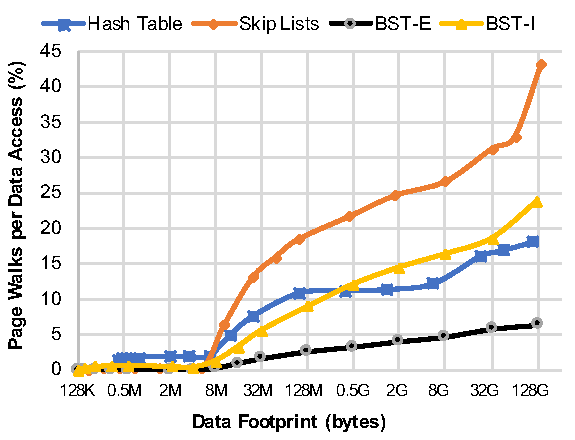
\includegraphics[width=1.0\columnwidth]{graphs/pagewalks.pdf}
   \caption{Frequency of page walks as a function of memory size.}
   \label{fig:pagewalks}
\end{figure}


\begin{table*}[]
\centering
\caption{Comparison of SpryVM with previous approaches for reducing virtual memory overhead.}
\label{table:vms}
\begin{tabular}{
>{\columncolor[HTML]{FFFFFF}}l |
>{\columncolor[HTML]{FFFFFF}}c |
>{\columncolor[HTML]{FFFFFF}}c |
>{\columncolor[HTML]{FFFFFF}}c |
>{\columncolor[HTML]{FFFFFF}}c |}
\cline{2-5}
\multicolumn{1}{c|}{\cellcolor[HTML]{FFFFFF}}                           & Programmability  & Performance and Efficiency & Flexibility & Safety and Security \\ \hline
\multicolumn{1}{|l|}{\cellcolor[HTML]{FFFFFF}Multi-page mappings~\cite{pham:colt, pham:increasing}}       & \cmark              & \xmark                          & \cmark           & \cmark      \\ \hline
\multicolumn{1}{|l|}{\cellcolor[HTML]{FFFFFF}Transparent Huge Pages~\cite{transparenthugepages}}    & \cmark               & \xmark                          & \cmark           & \cmark      \\ \hline
\multicolumn{1}{|l|}{\cellcolor[HTML]{FFFFFF}Libhugetlbfs~\cite{lighugetlbfs}}              & \xmark                & \xmark                          & \cmark           & \cmark      \\ \hline
\multicolumn{1}{|l|}{\cellcolor[HTML]{FFFFFF}Direct Segments~\cite{basu:efficient}}           & \xmark              & \cmark                          & \xmark           & \cmark      \\ \hline
\multicolumn{1}{|l|}{\cellcolor[HTML]{FFFFFF}Redundant Memory Mappings~\cite{karakostas:redundant}}  & \cmark             & \xmark                          & \xmark           & \cmark      \\ \hline
\multicolumn{1}{|l|}{\cellcolor[HTML]{FFFFFF}Direct-mapped Mappings~\cite{picorel:near-memory, haria:devirtualizing}}         & \cmark       & \cmark                          & \xmark           & \cmark      \\ \hline
\multicolumn{1}{|l|}{\cellcolor[HTML]{FFFFFF}SpryVM}                    & \cmark                       & \cmark               & \cmark           & \cmark      \\ \hline
\end{tabular}
\end{table*}

\subsection{Goals for VM in Heterogeneous Systems}
When buiding VM support for accelerators, it is important to identify
design goals for the its operation. Like prior work
\cite{haria:devirtualizing}, we identify the following as key goals in
our design:

\begin{itemize}
        \item \textbf{Programmability.} The widespread adoption of
          accelerators rests on the usability of and familiarity of
          their programming models. Unified virtual memory between
          CPUs and accelerators are one way of achieving this in a
          manner that simplifies data sharing, eliminating the need
          for hand-managed data copying and marshaling. Ideally, we
          wish to preserve all the benefits typically associated with
          VM like memory protection and isolation, and flexibility of
          sharing parts of the address space among processes, in a
          manner that is transparent and familiar to programmers.

        \item \textbf{Flexibility.} Traditional VM imposes no
          restrictions on virtual-to-physical page mapping
          relationships. This is valuable to support any level of
          system memory fragmentation, application multi-tenancy,
          memory allocation strategies transparent to programmers, as
          well as the integration of features such as demand-paging
          and copy-on-write (CoW). We wish to continue supporting this
          flexibility.

        \item \textbf{Safety and Security.} Direct access to physical
          memory is generally not acceptable nor desirable. Such
          memory management approaches cannot prevent malicious or
          erroneous memory accesses and prohibits sharing accelerators
          across different processes with proper
          isolation~\cite{haria:devirtualizing}. Furthermore, the
          entropy in address mapping must be as high as possible to
          reduce the vulnerability to security attacks.

        \item \textbf{Performance and Efficiency.} Crucially, all the
          goals listed thus far must be achievable without excessive
          performance or area overheads in hardware. In other words,
          address translation, the central mechanism on which VM's
          benefits rest, must provide near-zero performance overheads
          regardless of application working set and locality patterns,
          and must do so under tight area and power constraints. In
          the context of accelerators, the area and power budgets are
          even tighter because custom hardware is only integrated if
          it provides large performance benefits with minimal
          resources.


\end{itemize}


\subsection{Shortcomings of Modern MMU Hardware}
The ever-increasing memory needs of modern software has given rise to
scale-out systems with large memories that give low-latency access to
data \cite{ferdman:clearing, karakostas:performance, volos:fat,
  basu:efficient}. The advent of increasing memory sizes is
problematic for both address translation reach and latency, as we next
discuss.

\subsubsection{TLB Reach.}
Several studies have established the difficulties of building TLBs
with sufficient capacity or {\it reach} to cover increasing physical
memory sizes \cite{basu:efficient, haria:devirtualizing,
  pham:colt}. The common approach adopted by industry has been to
aggressively grow TLBs -- e.g., Intel has been doubling CPU TLBs from
Sandybridge to Skylake architectures -- and pay the cost of increased
area/power. Nevertheless, despite TLBs with thousands of entries, the
poor locality of access in emerging server workloads make TLB miss
rates problematic. Figure \ref{fig:pagewalks} captures this effect by
quantifying TLB miss rates as we vary the memory footprint of several
of our workloads on an Intel Broadwell chip with 1.5K-entry L2 TLBs
(see Section \ref{sec:methodology} for details). Despite Broadwell's
large thousand-entry TLBs, TLB miss rates imcrease dramatically with
larger memory footprints, corroborating results from prior work
\cite{basu:efficient}. Naturally, this poses big problems with the
advent of accelerators, which need their own TLBs. So far,
accelerators like GPUs have been equipped with massive
multi-thousand-entry TLBs too \cite{vesely:observation,
  lowepower:inferring}, but there is widespread consensus that this
approach is not viable for other more area-constrained accelerators
\cite{haria:devirtualizing, picorel:near-memory}. Perhaps even more
troublingly, while other techniques like large pages can offer partial
relief in some cases, they present their own set of challenges because
they offer only coarse-grained protection \cite{pham:large}, they can
be hard to form on fragmented systems \cite{kwon:coordinated}, they
have poor NUMA support \cite{gaud:large}, and they require complex TLB
hardware for concurrent page size support \cite{cox:efficient}. For
all these reasons, transparent support for large pages in OSes like
Linux only apply to 2MB pages (and not other sizes like 1GB) even
after decades of research \cite{arcangeli:transparent}.  Practically,
vendors implement multi-thousand-entry TLBs for the worst-case
scenario when base 4KB pages dominate. For the successful adoption, we
concur with recent work \cite{pham:colt, basu:efficient,
  karakostas:redundant, haria:devirtualizing} that alternate
approaches (complementary to large pages) to scalable TLB design are
needed.

\begin{comment}
As the memory capacity keeps increasing, TLB hit ratios decrease
sharply~\cite{basu:efficient} resulting in significantly higher
frequency of page walks. This effect is further exacerbated by
increasingly irregular access patterns of modern big data applications
that lack spatial and temporal
locality~\cite{haria:devirtualizing}. In response, modern systems have
embraced larger and more complex TLB hierarchies in an effort to
increase the TLB reach. However, increasing the TLB size beyond a few
dozen entries provides diminishing returns when accessing hundreds of
gigabytes of memory, especially in the absence of spatial and temporal
locality. Figure~\ref{fig:pagewalks} shows the number of page walks
per memory access as a function of the memory footprint for a set of
data traversal benchmarks running on an Intel Broadwell chip (for
methodology details, please refer to Section~{sec:methodology}). The
first thing to note that even large and deep TLB hierchies with >1.5K
TLB entries cannot deal with irregular traversals of large
datasets. The second thing to note is that the frequency of page walks
sharply increases with the size of the data. This result corroborates
a prior study on TLB ineffetiveness~\cite{basu:efficient}, which also
observed similar trends with larger pages sizes. While large pages are
highly effective in reducing translation overheads, they may not be
suitable for accelerators, and ultimately do not solve the problem as
memory continues to scale~\cite{basu:efficient}.

The area and power overheads of the translation hardware become
particularly concerning and impractical in heterogeneous systems with
a large number of tiny, highly customized
accelerators~\cite{haria:devirtualizing}, where the overheads of the
translation hardware can greatly surpass the power and area of the
rest of the functional parts of the accelerator. Given the increasing
gap between the memory growth and practical TLB capacity
growth~\cite{gandhi:badgertrap}, the TLB performance is certainly not
on a promising trajectory.

The underlying reason for poor TLB performance is that TBLs cache
translation on the execution side. Because of that, every execution
unit (be it a core or accelerator) must have a TLB unit, each of which
caches translations that cover the entire physical memory. This
becomes impractical, because the total amount of translation hardware
in the system grows linearly with the number of execution units, as
well as ineffective, because the memory growth makes each of the TLB
units incapable of achieving sufficient hit ratios. In contrast, if we
were able to design a system where TLBs would act as memory-side
translation caches, each serving one memory partition, then the number
of TLBs would not depend on the number of execution units. More
importantly, such TLBs would only need to cover a fraction of the
dataset, which would significantly increase their TLB hit ratios, as
per Figure~\ref{fig:pagewalks}.
\end{comment}

\subsubsection{Increasing Page Table Walk Latency.} 
In addition to TLB reach, the penalty of a TLB miss is critical to
address translation performance. For this reason, CPUs are equipped
with dedicated MMU caches to accelerate page table walks
\cite{bhattacharjee:large-reach, barr:translation}. Unfortunately,
even the presence of MMU caches cannot mitigate high page table walk
latencies in the context of accelerators. The key culprit is that
heterogeneous sytems with accelerators are usually integrated with
NUMA memories and require long-latency lookups across memory chips and
partitions. Even perfect MMU caches require at least one memory
reference per page table walk and recent work shows that this single
reference can dramatically exacerbate address translation costs for
accelerators \cite{picorel:near-memory}.


\subsection{Prior Approaches}

This part and Table~\ref{table:vms} overviews all prior work in memory management mechanism in terms of the aforesaid four goals presented before.

\noindent\textbf{Multi-page mappings.} Several studies exploited
the contiguity naturally generated by the buddy allocator and the
memory compactor. CoLT~\cite{pham:colt} and clustered~\cite{pham:increasing} TLBs coalesce 4-8 page translations into a single TLB entry, as long as their physical locations are contiguous. Although the TLB reach improves, it is still unable to cover the entirety of a large memory system of tens or hundreds of GBs~\cite{gandhi:range}, requiring large, deep, and power-hungry TLB hierarchies to cover all the memory.

\noindent\textbf{Huge pages.} The most common approach to increase the TLB reach is the introduction of larger page sizes by using Transparent Huge Pages (THP)~\cite{transparenthugepages} and libhugetlbfs~\cite{lighugetlbfs}. In commercial x86 and ARM architectures, 2MB and 1GB pages are supported in addition to the traditional 4KB page size. Unfortunately, the OS can only allocate huge pages when the available physical memory is size-aligned and contiguous, which is not possible when the system is under memory pressure. Furthermore, supporting multiple page sizes heavily increases the TLB hardware complexity, making huge pages unsuitable for area- and power-efficient accelerators.

\noindent\textbf{Segments.} More innovative ways of improving TLB coverage is the usage of variable-size segments instead of fixed page-based translations~\cite{karakostas:redundant, park:hybrid, basu:efficient}. Unfortunately, the effectiveness of these techniques relies on heavy changes to the OS's allocation path with at-allocation contiguity generation (i.e., eager paging). Furthermore, direct segments require applications to explicitly allocate a segment at startup, while redundant memory mappings (RMMs)~\cite{karakostas:redundant} requires highly associative power-hungry TLBs, both very unattractive from the programmability and hardware-efficiency perspectives.

\noindent\textbf{Direct-mapped mappings.} These techniques deliver almost near-zero overhead as they completely overlap translation with data fetch. Unfortunately, these techniques severely restrict the OS's memory allocation mechanism by either using identify mapping~\cite{haria:devirtualizing} or direct-mapped page-level allocation~\cite{picorel:near-memory}. The allocation restrictions limit the performance of such techniques with fragmented and application multi-tenancy scenarios, and complicate traditional OS mechanisms such as copy-on-write (COW) and the widely used fork system call optimization. Furthermore, these approaches drastically reduce the amount of entropy in address mapping, making the system more vulnerable to security attacks.


\javier{Points to come across:

\begin{itemize}
  \item SW trend: Servers workloads are keeping their datasets memory resident; HW trend: Due to slowdown in silicon density and efficiency, computer system are integrating custom logic (accelerators).
  \item Explain the programmability benefits of pointer-is-a-pointer AND flexible VM system (e.g., demand paging, COW) of a conventional translation mechanism.
  \item TLB Reach Problem: Explain that a conventional translation mechanism is not effective for accelerators because (1) it relies on deep cache and TLB hierarchies and (2) data reuse, to bridge the gap between computation speed and memory capacity. However, accelerators primarily exploit parallel access with proximity to memory, and not reuse and deep cache hierarchies. Furthermore, accelerator are custom and hence silicon optimized, hence the available budget for translation hardware is limited. I think we can just cite prior work on TLB miss rates for in-memory workloads.   
  \item TLB Penalty Problem: Explain that compute and memory are scaling-out due to the slowdown in silicon scaling and efficiency, hence TLB misses (page walks) become more costly. We can show something similar to Figure 1 here.
\end{itemize}


}


\section{Our Approach}
\label{our-approach}
Fundamentally, all prior techniques present the following maxim -- one
can either implement large power-hungry TLBs to accommodate all the
benefits of fully-flexible VM, or one can get away with smaller TLBs
as long as software flexibility is sacrificed. In the first scenario,
large TLBs are essential because VM is fully associative. In the
second scenario, software flexibility is sacrificed because VM imposes
restrictions reminiscent of direct mapping. DTRIM's contribution is
to showcase, however, that there is a third regime of operation
between these two extremes, where we implement set-associative VM to
continue enjoying the benefits of flexible VM without requiring large
TLBs. 

The core idea behind DTRIM is (partly) captured in Figure~\ref{fig:overview}. With
DTRIM, VM associativity is restricted in that a virtual page is
guaranteed to map to a physical page in a specific memory
``region'', but could reside anywhere within the region. This memory region could be a socket or a memory
channel. This effective set-associativity provides two
benefits. First, it enables us to replace large per-CPU/accelerator
TLB that need to address the entire physical address space with
memory-side TLBs responsible for mapping only their specific memory
regions. Because memory regions represent just a subset of the total
physical address space, memory-side TLBs can achieve high hit rates
despite being smaller in size. Second, set-associativity also permits
us to dramatically reduce TLB miss penalty by allowing co-location of data and
the corresponding translations in the same memory regions, overlapping their
lookup. The confluence of these two benefits is a combination of
better performance and reduction in TLB resources. 

A factor in our approach is that implementing set-associativity in a
commodity OS requires only modest changes to existing memory
allocation/management code-paths. Furthermore, we have found that in
practice, we can achieve good address translation performance by only
modestly reducing associativity from the default fully-associative VM
approach. Consequently, DTRIM implements unified CPU-accelerator
address spaces without forcing coarser-grained memory protection,
compromising on entropy in virtual address bits, or requiring
power/area-hungry TLBs. The fact that DTRIM does not rely on
contiguity also means that it can continue to operate efficiently in
fragmented memory settings where translation contiguity or identity
mappings may be hard to generate. Furthermore, having only a modest drop
from fully-associative designs means that optimizations like
copy-on-write can, for all practical purposes, can be supported (we will
show that the number of CoW pages is limited only by the size of the
memory region, which can be thousands of pages in practice).




\begin{figure*}
\centering
 \subfloat[Memcached --- 1 Process]{
  \label{fig:memcached_1p}
%  \includegraphics[width=.32\textwidth,clip,trim = 18mm 213mm 117mm 20mm]{figs/eps/sim-rread-lat.eps}}
   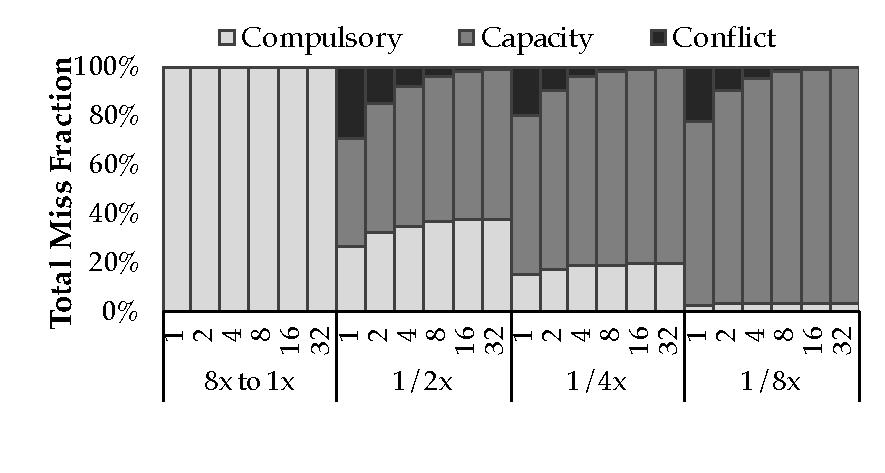
\includegraphics[width=.365\textwidth,clip]{graphs/memcached_assoc_1p-bw.pdf}}
%  \hspace{.01in}
 \subfloat[RocksDB --- 1 Process]{
  \label{fig:rocksdb_1p}
%  \includegraphics[width=.32\textwidth,clip,trim = 18mm 213mm 115mm 20mm]{figs/eps/sim-rread-bw.eps}}
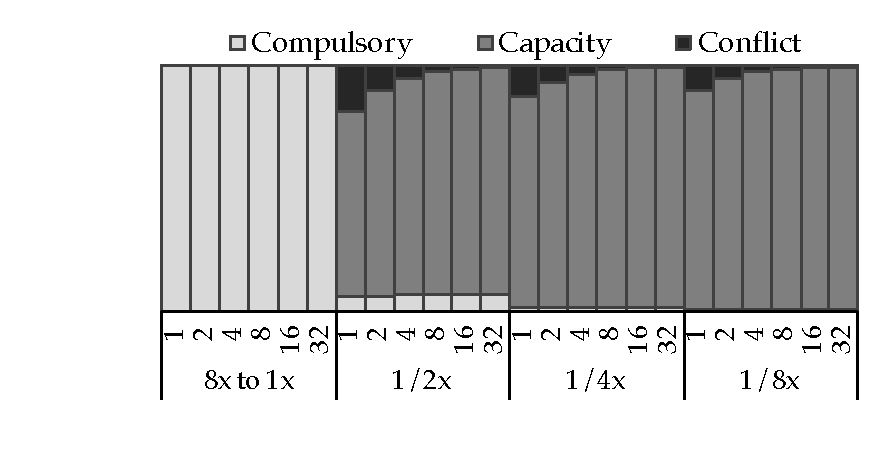
\includegraphics[width=.31\textwidth,clip]{graphs/rocksdb_assoc_1p-bw.pdf}}
%   \hspace{.01in}
 \subfloat[Cassandra --- 1 Process]{
  \label{fig:cassandra_1p}
%  \includegraphics[width=.32\textwidth,clip,trim = 28mm 217mm 115mm 20mm]{figs/eps/emu-rread-lat_cropped.eps}}
  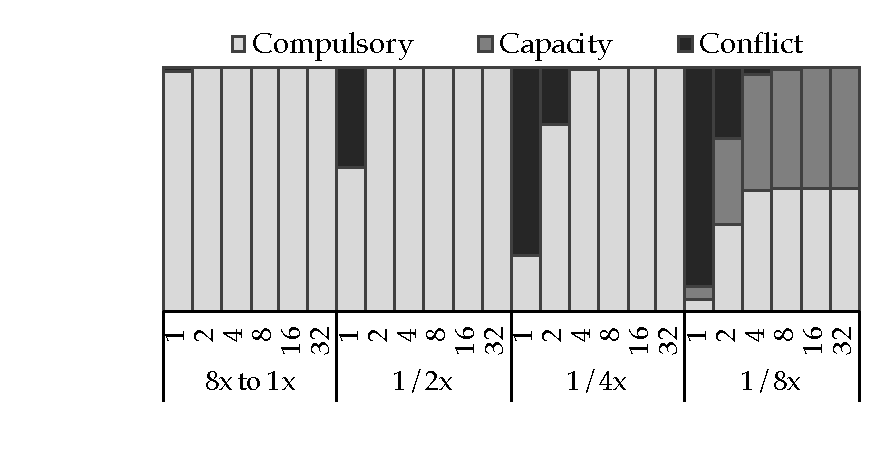
\includegraphics[width=.31\textwidth,clip]{graphs/cassandra_assoc_1p-bw.pdf}}
\caption{Overall miss ratio broken down into compulsory, capacity, and conflict misses.
 \label{fig:miss_ratio}}
\end{figure*}

%\section{Associativity in Virtual Memory}
\section{SpryVM}
\label{sec:associativity}

%\javier{ Points to come across:
%
%\begin{itemize}
%  \item We can have a first subsection to talk about the 4 points of the intro's table (i.e., programmability, power/perf, flexibility, safety). What we would like to have, the goal. 
%  \item We can have second subsection to talk about the problems of full associativity, and the idea of set associativity, which is essentially partitioning the memory and translation information and knowing to which memory set to go, and how that can help at the aforesaid 4 points. We can have a high-level figure on how the memory and the translation information is partitioned. 
%  NOTE: This section has to be short, maximum one page, and zero results! It has to be high level!!!
%\end{itemize}

%}

In this section, we provide a high-level description of the SpryVM scheme. We start by enumerating the set of goals of an ideal memory management mechanism, continue with prior work and how it falls short of achieving all the aforesaid goals, and finally we introduce SpryVM and how our approach is able to achieve all the desired requirements.

\subsection{Ideal goals for memory management}

For the list of goals, we decided to follow prior work's classification~\cite{haria:devirtualizing} for an homologated comparison.

\begin{itemize}
	\item \textbf{Programmability.} The widespread adoption of heterogeneous architectures depends on the usability of their programming models. A crucial step in addressing this challenge is to enable unified VM across CPUs and accelerators. This model makes any pointer equally valid everywhere~\cite{hsa}, simplifying data sharing, and eliminating the need for explicit data copies and manual data consistency maintenance. Additionally, VM enables transparent memory allocation and protection, providing the familiar programming environment that programmers expect.
	\item \textbf{Area and Power.} An ideal memory management mechanism should provide near-zero overhead with any working set size and data locality characteristics under tight area and power constraints. In the context of accelerators, these area and power budgets are even tighter because custom hardware is only integrated if it provides large performance benefits with minimal resources. 
	\item \textbf{Flexibility.} Memory management schemes should not overly restrict the VM mappings to become efficient. This way they are widely applicable to any levels of fragmentation and application multi-tenancy. Furthermore, schemes should not break traditional OS mechanisms such as demand-paging and copy-on-write (COW), which prevent the use of well-established optimization techniques.  
		
	\item \textbf{Safety.} Direct access to physical memory is generally not acceptable nor desirable. Such memory management approaches cannot prevent malicious or erroneous memory accesses and prohibits sharing accelerators across different processes with proper isolation.
\end{itemize}

\subsection{Memory management mechanisms}

This part and Table~\ref{table:vms} overviews all prior work in memory management mechanism in terms of the aforesaid four goals presented before. 

\noindent\textbf{Multi-page mappings.} Several studies exploited
the contiguity naturally generated by the buddy allocator and the
memory compactor. CoLT~\cite{pham:colt} and clustered~\cite{pham:increasing} TLBs coalesce 4-8 page translations into a single TLB entry, as long as their physical locations are contiguously in memory. Although the TLB reach improves, it is still unable to cover the entirety of a large memory system of tens or hundreds of GBs~\cite{gandhi:range}, requiring large, deep, and power-hungry TLB hierarchies to cover all the memory. 

\noindent\textbf{Huge pages.} The most common approach to increase the TLB reach is the introduction of larger page sizes by using Transparent Huge Pages (THP)~\cite{transparenthugepages} and libhugetlbfs~\cite{lighugetlbfs}. In commercial x86 and ARM architectures, 2MB and 1GB pages are supported in addition to the traditional 4KB page size. Unfortunately, the OS can only allocate huge pages when the available physical memory is size-aligned and contiguous, which is not possible when the system is under memory pressure. Furthermore, supporting multiple page sizes heavily increases the TLB hardware complexity, making huge pages unsuitable for area and power efficient accelerators.

\noindent\textbf{Segments.} More innovative ways of improving TLB coverage is the usage of variable-size segments instead of fixed page-based translations~\cite{karakostas:redundant, park:hybrid, basu:efficient}. Unfortunately, the effectiveness of all these techniques relies on heavy changes to the OS's allocation path with at-allocation contiguity generation (i.e., eager paging). Furthermore, direct segments requires applications to explicitly allocate a segment at startup, while redundant memory mappings (RMMs)~\cite{karakostas:redundant} requires highly associative power-hungry TLBs, both very unattractive from the programmability and hardware-efficiency perspectives. 

\noindent\textbf{Direct-mapped mappings.} These techniques deliver almost near-zero overhead as they completely overlap translation with data fetch. Unfortunately, these techniques severely restrict the OS's memory allocation mechanism by either using identify mapping~\cite{haria:devirtualizing} or direct-mapped page-level allocation~\cite{picorel:near-memory}. The allocation restrictions limit the performance of such techniques with fragmented and application multi-tenancy scenarios, and complicate traditional OS mechanisms such as copy-on-write (COW) and the widely used fork system call optimization.

\subsection{Reducing associativity in Virtual Memory}

As shown before, there is no single memory management mechanism that achieves all the desired goals. Most importantly, we have seen that there is a tradeoff between VM flexibility and hardware complexity; the more restricted the OS's memory allocation path is, the lower the hardware complexity required to achieve competitive performance is. More specifically, we observe that traditional VM require large TLBs because it is fully associative (i.e., a virtual page can potentially map to any physical frame). In contrast, VM techniques that exhibit minimal TLB requirements by creating vast virtual-to-physical contiguity~\cite{basu:efficient, gandhi:range, haria:devirtualizing} impose strong restrictions on which page frames to assign to a virtual page, reminiscent of the notion of direct-mapping. 

Alternatively to all prior work, our approach is to find a middle-ground between these techniques and propose set-associative VM, where a virtual page can map to one among a set of page frames. We name this approach spryVM (Set-Associative Regions of Your Virtual Memory). SpryVM slightly restricts VM associativity so that a virtual address uniquely
identifies the region of the physical address space (e.g., a socket and memory channel)
that holds the data and performs translation using per-region TLBs. This insight
facilitates area-efficient TLBs with high hit rates (because separate
TLBs are responsible for disjoint parts of the physical address space)
and fast miss penalties (because spryVM can co-colate both translation
and data in TLB's physical partition, their lookup can be
overlapped). Importantly, we show that the OS support necessary to
achieve this approach is compatible with existing OSes and does not
sacrifice flexibility like in prior work. \javier{I need a figure to explain SpryVM in a little more detail.}

\noindent\textbf{Programmability.} SpryVM enables a unified Virtual Memory layer for CPUs and accelerators has many benefits: a simpler programming model, enabling "a pointer is a pointer everywhere" semantics~\cite{pichai:architectural, power:supporting, vesely:observation}, extending memory protection to accelerators, and obviating the need for manual inter-CPU-accelerator data marshalling.  

\noindent\textbf{Area and Power.} SpryVM performs address translation using per-region TLBs. Our TLBs are area-efficient due to both high hit rates and a fast miss penalty. The high hit rates are because of having seperate TLBs being responsible for disjoint parts of the physical memory, increasing TLB reach and locality. SpryVM achieves fast TLB miss penalty by having each region holding the data and translation information, which allows to overlap most of the translation and data fetch time.


\noindent\textbf{Flexibility.} SpryVM slightly restricts the VM associativity so that a virtual page uniquely identifies a region in the physical memory space (e.g., a socket and a memory channel). This mapping delivers great flexibility as current systems integrate 10s to 100s of GB of memory, translating into a flexibility of 10s to 100s of millions of page frames that a virtual page can potentially map to. More importantly, we show that the OS support necessary to achieve this approach is compatible with existing OSes and does not sacrifice flexibility, allowing demand-paging and COW optimizations~\footnote{The number of COW pages is limited by the size of the memory partition.}.

\noindent\textbf{Safety.} In SpryVM, accelerators require address translation to access the target page frame and check the permissions, like in conventional VM. Hence, SpryVM provides protection for malicious and erroneous data accesses and facilitates sharing accelerators across multiple processes.

 
%In modern page-based VM, a virtual page is mapped on demand into a page frame. Modern systems place no restrictions on the virtual-to-physical mapping; a virtual page can potentially map to any page frame. Though flexible, this fully associative approach places translation on the critical path of every memory access, because a memory access cannot begin until the translation operation finishes.

%One potential way to break translation-memory access serialization is to completely eliminate associativity and enforce a direct mapping between virtual pages and page frames. Since a virtual page can now only map to a single page frame, address translation and data fetch are independent and can proceed in parallel. Conventional wisdom dictates that direct mapping creates an excess of page faults, due to conflicts from multiple virtual pages mapping to the same page frame. However, this is merely intuition, as there exists no study on VM associativity, unlike caches, which are similar in some organizational aspects and for which such a study has existed for three decades~\cite{hill:aspects}. 

%%%%%%%%%%% Table: Methodology %%%%%%%%%%%
\begin{table}
 \begin{center}
  \caption{Workload description.}
  \scalebox{0.7}
  \small
  \vspace{0.01in}
  \label{table:workload}
  \renewcommand{\arraystretch}{1.0}
   {\scriptsize
    \begin{tabular}{ l  l }
     %\hline
     \toprule
      {\bf Workload}                  & {\bf Description}  \\
     	%\hline
     	%\hline
     	\toprule
      	\multirow{1}{*}{Cassandra}                       &  NoSQL data store running Yahoo's YCSB. \\
     	%\hline
     	\cmidrule{2-2}
      	\multirow{1}{*}{Memcached}                      & Cache store running Twitter-like workload~\cite{lim:thin}. \\
     	%\hline
	\cmidrule{2-2}
        %\multirow{2}{*}{Core Types}    & In-order (Cortex A8-like): 2-wide \\
	%		                               &  OoO (Xeon-like): 4-wide, 128-entry ROB \\
	%\hline
		\multirow{1}{*}{TPC-H}	& TPC-H on MonetDB column store (Q1-Q21). \\
	\cmidrule{2-2}
		\multirow{1}{*}{TPC-DS}	& TPC-DS on MonetDB column store (Queries of~\cite{kocberber:meet}). \\
		\cmidrule{2-2}
	%\multirow{2}{*}{L1-I/D Caches}	&	32KB, split, 2 ports, 64B blocks, 10 MSHRs, \\
	%							& 2-cycle load-to-use latency \\
	 	\multirow{1}{*}{MySQL} 			& SQL DBMS running Facebook's LinkBench~\cite{facebook:linkbench}. \\
	%\hline
     \cmidrule{2-2}
      \multirow{1}{*}{RocksDB}                             &  Store engine running Facebook benchmarks~\cite{facebook:rocksdb}. \\ %a canonical uniform request distribution. \\
      %\hline

     \bottomrule
     %\hline
    \end{tabular}
   } %small
 \end{center}
  \vspace{-0.1in}
\end{table}
%%%%%%%%%%% END Table: Methodology %%%%%%%%%%%%

%To fill this research void, we employ the 3C model---initially developed for caches~\cite{hill:aspects}---to study VM associativity. In this context, associativity means the number of possible locations (page frames) a given virtual page can map to. This model classifies misses (i.e., page faults) into three categories: conflict misses (when too many active pages map to a fraction of the sets), capacity misses (due to limited memory size), and compulsory misses (upon the first access to a page). 

%To simulate real-world scenarios, we select a set of representative server workloads, summarized in Table~\ref{table:workload}. We include two cloud workloads from CloudSuite~\cite{ferdman:clearing}, Cassandra and Memcached, an online transaction processing (OLTP) workload~\cite{facebook:linkbench}, MySQL, two online analytical processing (OLAP) workloads~\cite{boncz:breaking}, TPC-H and TPC-DS, and a widely-used storage system workload~\cite{dong:optimizing}, RocksDB. We collect long memory traces of several 10s of billions of instructions of the server workloads using Pin~\cite{luk:pin}. We extract the virtual address and address space identifier (ASID) of each memory reference and use it to probe a set-associative memory structure, varying the associativity to observe and classify the misses. A detailed description of our methodology is found in Section~\ref{sec:methodology}.

%\subsection{Single-Process In-Memory}

%Fig.~\ref{fig:miss_ratio} shows results for three single-process workloads: Memcached, RocksDB, and Cassandra. The y-axis breaks down the total misses into the three distinct miss classes. Each category on the x-axis corresponds to the ratio between the size of the physical memory and the size of the application's working set. For example,  $8\times$ indicates that the memory is eight times larger than the application's working set. Similarly, $1/2\times$ means that the application's working set is twice the size of the memory. We collapse results for $8\times$ to $1\times$ because they are similar and visually identical; each case represents a fully in-memory scenario. Furthermore, within each working set category, the x-axis sweeps through different VM associativities, from direct-mapped to 32-way associative. 

\begin{figure*}[t]
\centering
 \subfloat[Memcached --- 2 Processes]{
  \label{fig:memcached_2p_assoc}
  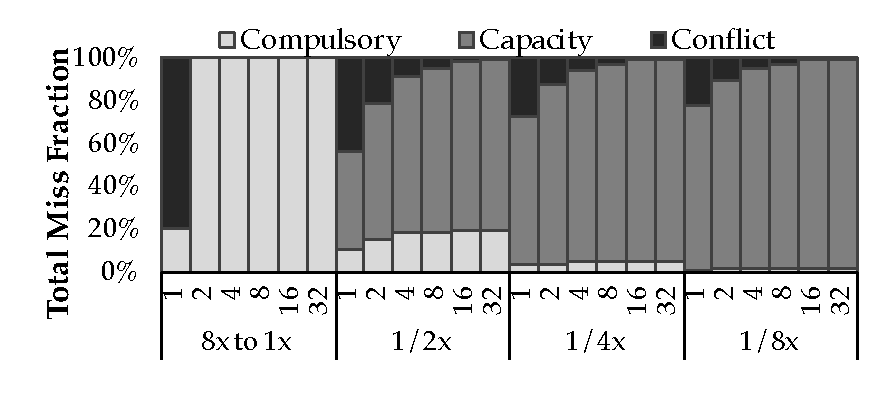
\includegraphics[width=.36\textwidth,clip]{graphs/memcached_assoc_2p-bw.pdf}}
 \subfloat[Memcached --- 4 Processes]{
  \label{fig:memcached_4p_assoc}
 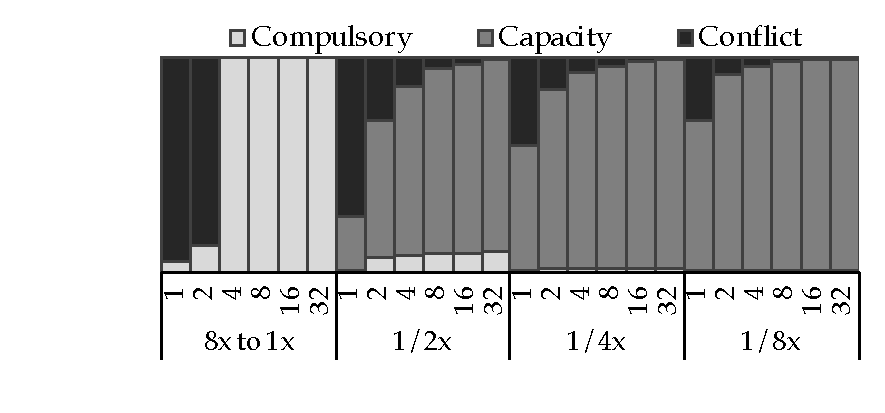
\includegraphics[width=.31\textwidth,clip]{graphs/memcached_assoc_4p-bw.pdf}}
 \subfloat[Memcached --- 8 Processes]{
  \label{fig:memcached_8p}
  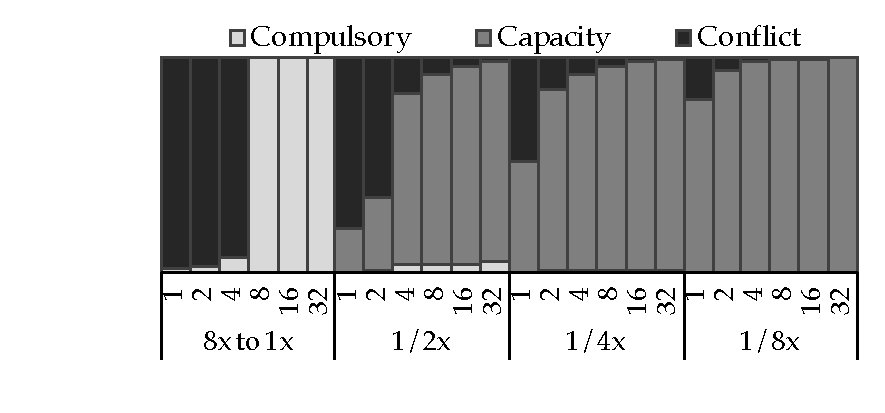
\includegraphics[width=.31\textwidth,clip]{graphs/memcached_assoc_8p-bw.pdf}}
 \hspace{.01in}
 \subfloat[RocksDB --- 2 Processes]{
  \label{fig:rocksdb_2p}
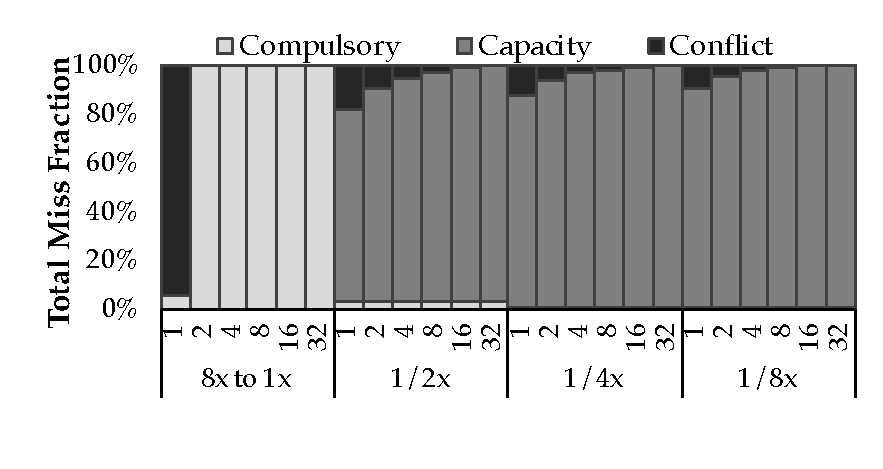
\includegraphics[width=.36\textwidth,clip]{graphs/rocksdb_assoc_2p-bw.pdf}}
  \subfloat[RocksDB --- 4 Processes]{
  \label{fig:rocksdb_4p}
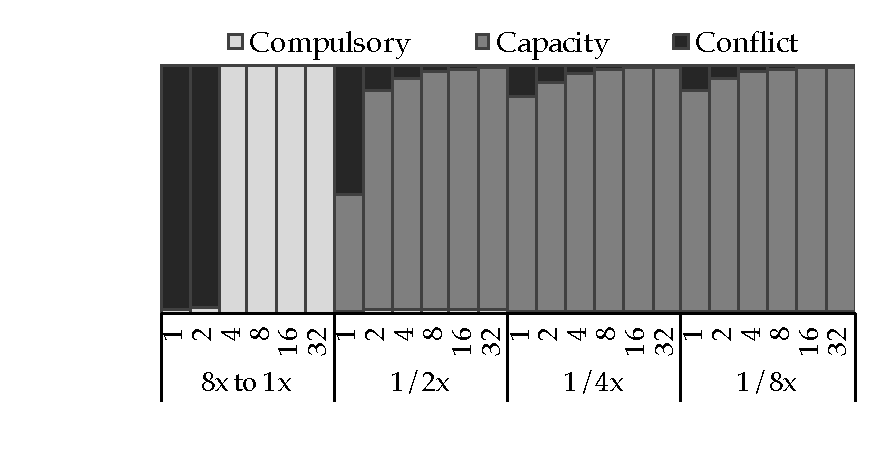
\includegraphics[width=.305\textwidth,clip]{graphs/rocksdb_assoc_4p-bw.pdf}}
  \subfloat[RocksDB --- 8 Processes]{
  \label{fig:rocksdb_8p}
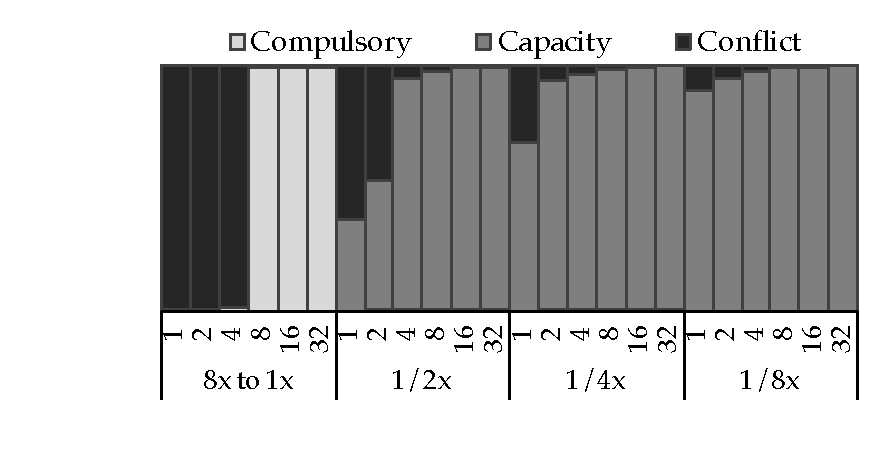
\includegraphics[width=.31\textwidth,clip]{graphs/rocksdb_assoc_8p-bw.pdf}}
  \hspace{.01in}
 \subfloat[Cassandra --- 2 Processes]{
  \label{fig:cassandra_2p}
  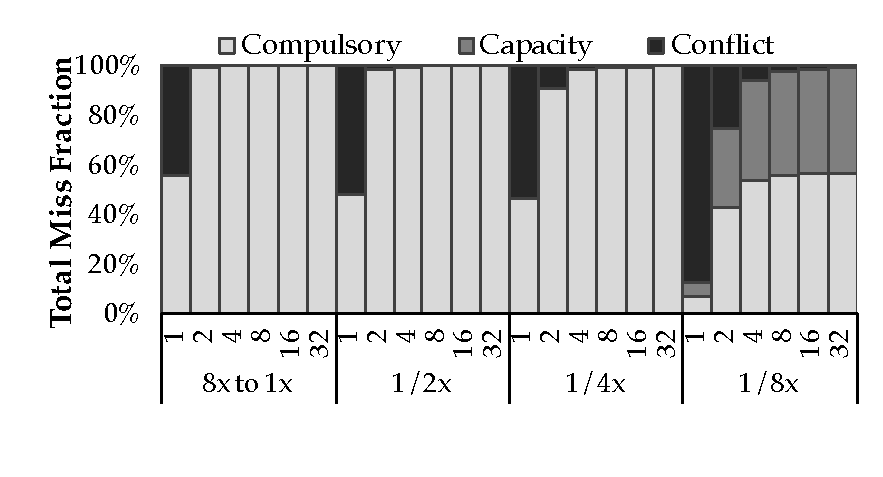
\includegraphics[width=.355\textwidth,clip]{graphs/cassandra_assoc_2p-bw.pdf}}
  \subfloat[Cassandra --- 4 Processes]{
  \label{fig:cassandra_4p}
  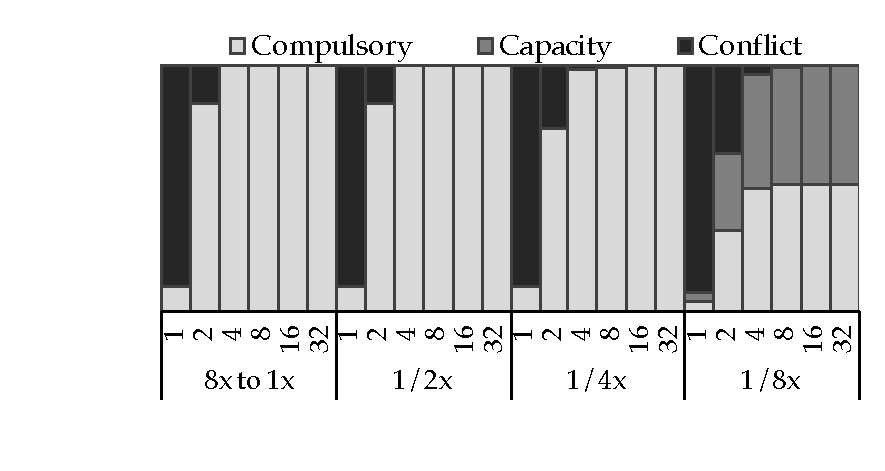
\includegraphics[width=.31\textwidth,clip]{graphs/cassandra_assoc_4p-bw.pdf}}
  \subfloat[Cassandra --- 8 Processes]{
  \label{fig:cassandra_8p}
  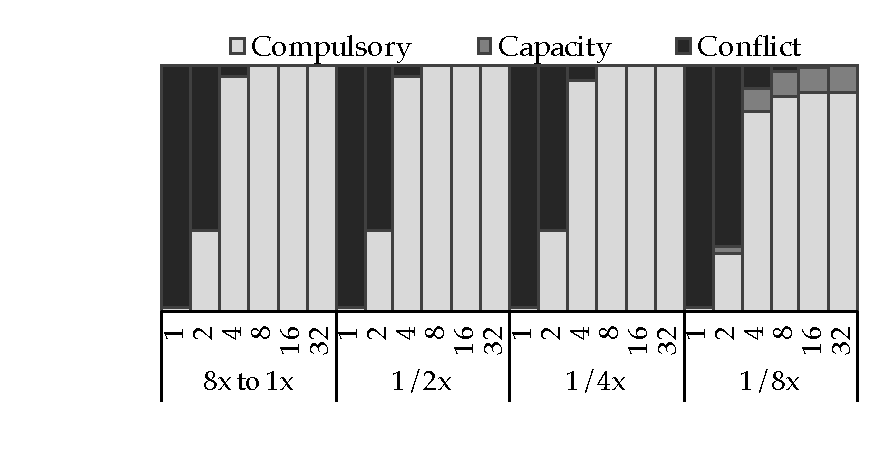
\includegraphics[width=.31\textwidth,clip]{graphs/cassandra_assoc_8p-bw.pdf}}


\caption{Overall miss ratio broken down into compulsory, capacity, and conflict misses.
 \label{fig:miss_ratio_procs}}
\end{figure*}


%Even with a simple direct-mapped translation, compulsory misses represent $99.9\%$ of all the misses. There are no capacity misses as the working set fully fits in memory. Conflict misses are scarce. For example, Memcached using direct-mapped translation achieves a conflict miss rate in the order of one miss per $10^{8}$ memory accesses. Using $2$ ways removes all the conflicts for the $8\times$, $4\times$, and $2\times$ cases, while $4$ ways are required for the $1\times$ case (where the memory size is equal to the size of the working set). For in-memory scenarios, page conflicts arise because the virtual address space of server applications is particularly sparse; there are many virtual segments scattered all over the address space. For example, Java processes exhibit many virtual segments due to the dynamic nature of the JVM. This is best observed in the case of Cassandra, which exhibits direct-mapped conflict miss rates in the order of one miss per $10^{7}$ and $10^{6}$ memory accesses for the $8\times$--$2\times$ cases and the $1\times$ case respectively. However, conflict misses drop rapidly as associativity increases and using 4 ways removes all conflicts for the $4\times$ and $2\times$ cases, while virtually eliminating conflicts for the $1\times$ case. The observation that conflict misses drop rapidly with associativity has also been shown for caches~\cite{hill:aspects, cantin:cache}. We elide the results for TPC-H, TPC-DS, and MySQL as they follow identical trends.

%\subsection{Single-Process Out-of-Memory}

%In contrast to in-memory scenarios, when the working sets do not fit in memory ($1/2\times$, $1/4\times$, $1/8\times$ cases), capacity misses grow with the working set size, while the fraction of compulsory misses drops. Although conflict misses are more significant than in the in-memory scenarios, conflicts drop sharply after 2-4 ways. In the worst case, 16 ways are required to drive conflict misses down to $\sim1\%$ of all the misses. Note that Cassandra has an active working set that fits in a memory of $1/4\times$ the data size, and capacity misses start to rise at the $1/8\times$ case and beyond. Fundamentally, all these results corroborate the seminal work on caches~\cite{hill:aspects, cantin:cache}. 

%\subsection{Multi-programming In-Memory}
%Fig.~\ref{fig:miss_ratio_procs} presents results for multi-programming. We take each of the three workloads, Memcached, RocksDB, and Cassandra, and increase the number of processes, keeping the overall working set size the same with respect to the single process scenarios. For example, for the $1\times$ case in Fig.~\ref{fig:miss_ratio}, the working set of a single process equals the size of the memory. In Fig.~\ref{fig:miss_ratio_procs}, for two processes sharing the same physical memory, the per-process working set is half the size of the physical memory. Similarly, with four processes, per-process working sets consume a quarter of the physical memory. We thus guarantee that only the increase in the number of processes has an impact on the associativity. 

%For in-memory scenarios ($8\times$--$1\times$ cases), once the associativity equals the number of processes, compulsory misses represent $99.9\%$ of all the misses for all the workloads. Increasing the associativity further makes conflicts virtually disappear after a few additional ways. For instance, for Memcached, with 8, 16, and 32 ways, the conflicts are in the order of a single miss per $10^{9}$ accesses for 2, 4, and 8 processes, respectively. Cassandra requires 4, 8, and 8 ways to achieve a miss conflict rate of one miss per $10^{9}$ accesses for 2, 4, and 8 processes, respectively. Again, the trends are identical for TPC-H, TPC-DS, and MySQL. Overall, conflict misses become virtually zero with a few ways (i.e., 2-4) per process.

%%%% THINK WHETHER TO ADD THIS
%Although Fig.~\ref{fig:miss_ratio} and \ref{fig:miss_ratio_procs} show results that use the standard method of computing the index by using the least-significant bits of the VPN, we also studied an alternative proposal whose strength is distributing address more evenly over sets~\cite{qureshi:fundamental}. It did not reduce conflicts significantly due to the fact that page conflicts arise when many pages map to the same memory set, even when assuming a uniform page distribution. Changing the index function uniformly changes the distribution, and therefore does not mitigate the issue. Once again this behavior corroborates prior work on caches~\cite{hill:aspects}.

%\subsection{Multi-programming Out-of-Memory}

%For the cases where the working sets do not fit in memory, the trends are similar to the single-process scenarios. Capacity misses become more significant as the working set sizes grow, making conflict and compulsory misses less important. Similar to the in-memory case, once the associativity equals the number of processes, the fraction of conflict misses matches the single-process results. Conflicts drop rapidly as in the other cases and with 4 ways per process, conflict misses remain within $1\%$ of the total misses for all the workloads. The results for TPC-H, TPC-DS, and MySQL are identical.

%\subsection{Observations \& Implications}

%Our results show that fully associative VM is unnecessary for many modern server workloads. This observation holds across scenarios that span single process, multi-programming, in-memory and out-of-memory working sets. Compulsory and capacity misses dominate, and conflict misses, which associativity alleviates, drop rapidly as the associativity increases. Specifically, for in-memory scenarios, compulsory misses dominate when associativity equals the number of processes. For out-of-the-memory scenarios, capacity misses dominate and become more important as working set sizes increase. In this case, conflict misses become scarce once associativity matches the number of processes, and virtually disappear after a few extra ways. These trends match prior literature on caches~\cite{hill:aspects, cantin:cache, hill:case}---just as set-associative (or direct-mapped) caches can often provide nearly all the benefits of full associativity with faster access times, set-associative VM can provide nearly all the benefits of full associativity with faster translation. 

%To put the associativity requirements into perspective, a commodity server today integrates $256$GB of memory~\cite{ning:open}. Assuming $4$KB pages, fully associative VM provides $64M$ ways. As there are around $100$ processes concurrently running after booting~\cite{ahn:revising}, even when assuming a system with 128 processes and an associativity of 16 per process---which is extreme as we have seen that an associativity of 2--4 per process is sufficient---the total associativity requirements does not exceed $2K$ ways. Even for a commodity server, the $2K$ requirement is $32K\times$ less than what full associativity provides. A server with a larger memory capacity (e.g., large NUMA machines~\cite{hp:hp, huawei:kunlun}) or with emerging non-volatile memories (e.g., 3D XPoint~\cite{3dxpoint}) would supply even more ways, widening the gap between the required and provided associativity. 




%\section{DTRIM}
\label{sec:msmmu}

\javier{Points to come across:

\begin{itemize}
  \item Implementation and how it tackles the TLB reach and penalty.
  \item We need figures explaining how the translation works with steps. 
\end{itemize}

}

In this section, we investigate the design space for address translation for MPUs, given the modest associativity requirements and the characteristics of our memory-chip network. Then, we propose and describe our solution, DTRIM.

\subsection{Placement}

A straightforward extension of address translation to MPUs integrates an MMU in each MPU. Each MPU probes its MMU on each memory access, and upon a miss in its TLBs, initiates a conventional page table walk. Fig.~\ref{fig:baseline} shows a page walk that references a page table entry residing in another memory chip and partition, which is the common case in systems with multiple chips and partitions. Blue arrows indicate translation-related memory messages, while red arrows show data fetch. %In other words, memory accesses to page table entries are colored in blue, while accesses to page frames are red. 

\begin{figure}[h!]
\centering
 \subfloat[Baseline.]{
  \label{fig:baseline}
%  \includegraphics[width=.32\textwidth,clip,trim = 18mm 213mm 117mm 20mm]{figs/eps/sim-rread-lat.eps}}
   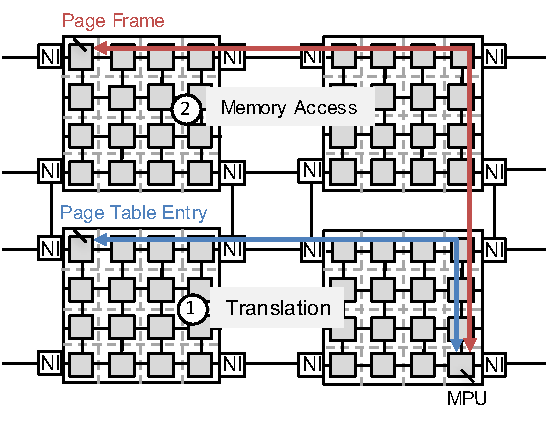
\includegraphics[clip,width=0.75\columnwidth]{figures/floorplan_vanilavm2.pdf}
%   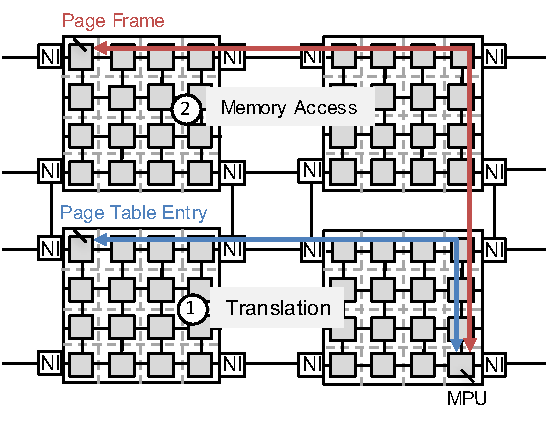
\includegraphics[width=0.69\columnwidth]{figures/floorplan_vanilavm2.pdf}}
   }
%  \hspace{.01in}

 \subfloat[Per-Chip MMU.]{
  \label{fig:chipmmu}
%  \includegraphics[width=.32\textwidth,clip,trim = 18mm 213mm 115mm 20mm]{figs/eps/sim-rread-bw.eps}}
 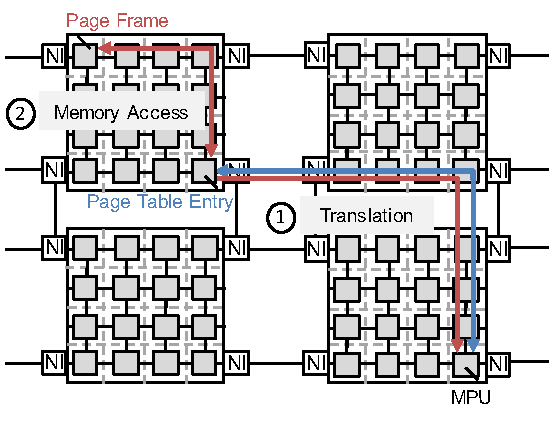
\includegraphics[clip,width=0.75\columnwidth]{figures/floorplan_chipvm2.pdf}
 %  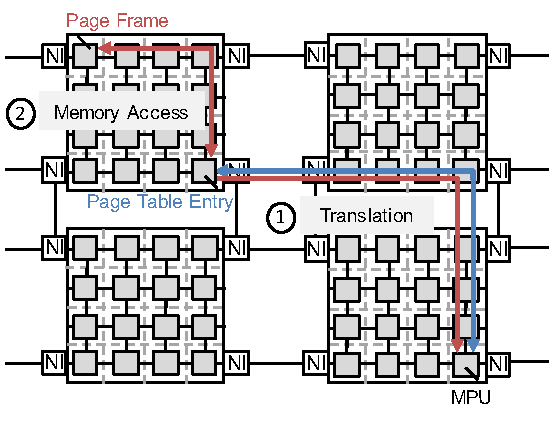
\includegraphics[width=0.69\columnwidth]{figures/floorplan_chipvm2.pdf}}
 }
% \hspace{.01in}

 \subfloat[Per-Partition MMU.]{
  \label{fig:partitionmmu}
%  \includegraphics[width=.32\textwidth,clip,trim = 18mm 213mm 115mm 20mm]{figs/eps/sim-rread-bw.eps}}
 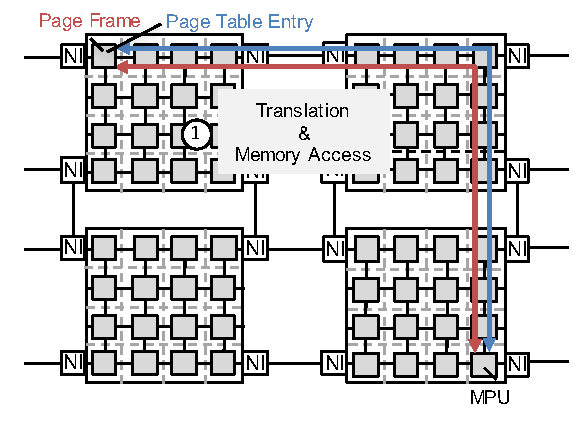
\includegraphics[clip,width=0.75\columnwidth]{figures/floorplan_partitionvm2.pdf}
%  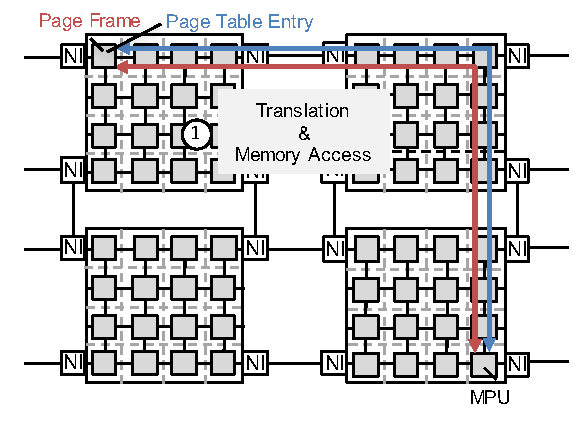
\includegraphics[width=0.695\columnwidth]{figures/floorplan_partitionvm2.pdf}}
 }

\caption{Different translation schemes on 4-chip floor plans. Large squares and small gray squares represent memory chips and partitions, respectively. Translation and memory access messages appear in blue and red, respectively. 
 \label{fig:translationSchemes_comparison}}
\end{figure}

There are several problems with this baseline. First, the page table entry that contains the physical address can be anywhere in the system, involving expensive interconnect traversals which makes page walks costly. Second, the data fetch cannot begin until the translation operation finishes, adding the translation latency to the data fetch latency. Third, the translation process does not finish until the page table entry returns to the MPU, even if the page table entry and the target page frame are in the same chip or memory partition. The fundamental problem is that there is no direct relation between virtual page numbers and page frames, something inherent to fully associative VM. The consequence is that there is no expected correlation between the location of page table entries and page frames, precluding fetching the data before the page table entry returns to the MPU. Although this design makes sense for fully associative VM, it is not optimal for set-associative VM.

We now exploit the modest associativity requirements and consider memory sets that span a memory chip only. A virtual address identifies a memory chip uniquely, and hence we know that the target page frame is somewhere in that chip. Under this constraint, we can utilize a centralized per-chip MMU, along with a page table and a set of TLBs, as shown in Fig.~\ref{fig:chipmmu}. Upon a page walk operation from an MPU, the virtual address is used to access the per-chip MMU. If the translation is not in the per-chip TLBs, a page walk in the memory chip begins. When the page walk finishes, the MMU in the memory chip starts the data fetch immediately, referencing the page frame (which can reside in any of the partitions in the chip). When the data returns to the per-chip MMU, both the page table entry and data return to the MPU. 

This method is an improvement over the baseline for two reasons. First, translation and data fetch overlap the latency on the interconnect to reach the target memory chip, as only the virtual address is used to locate the memory chip. Second, the translation process finishes as soon as the page walk within the memory chip finishes. However, there is room for improvement. As the virtual address only identifies the memory chip, page frames and page table entries can be in any memory partition. This placement creates two problems. First, the centralized per-chip MMU can be located anywhere in the chip, and upon a page walk, the page table entry could be located in a different partition. Second, the target page frame might also be located in another partition. Based on the latency results of Fig.~\ref{fig:e2elat}, the overhead could be significant. 

Going beyond, we can co-locate the page table entries and the page frames in the same memory partition, where memory accesses are faster, and employ a per-partition MMU. In this case, shown in Fig.~\ref{fig:partitionmmu}, memory sets only encompass a memory partition. The locality-aware placement of the MMU delivers the best performance among all. First, the translation and data fetch operations overlap the latency to reach the memory partition---because only the virtual address is used to locate the memory partition. Second, the translation finishes as soon as the page walk within the memory partition finishes, and since the target page frame is within the same partition, the data fetch can begin immediately (without traversing any interconnect).

\subsection{Page Table}
\label{sec:pagetable}

After defining the location of the memory-side MMUs, the next step is to choose a page table. Although there are many page table implementations~\cite{yaniv:hash}, we choose an inverted page table for the following reasons. First, inverted page tables do not need to be dynamically resized, so they are allocated once and pinned contiguously in memory~\cite{jacob:look}. Second, all the processes whose pages map to the partition share the same page table. Finally, when there are no collisions in the inverted page table, page walks only require a single memory access.

One of the key parameters of an inverted page table is the ratio between the number of page frames and page table entries, also called the load factor~\cite{cormen:introduction}. The load factor directly dictates the rate of collisions (i.e., the frequency of two virtual page numbers mapping to the same page table entry). Importantly, given a load factor, the collision rate is not affected by the working set size or access patterns, assuming uniform hashing~\cite{cormen:introduction}. In Fig.~\ref{fig:memref}, we compare a conventional modulo hash to a stronger k-bit XOR folding~\cite{qureshi:fundamental}, to demonstrate the effects of hashing on page table collisions. As we have not seen significant differences in workloads, process counts, and memory size to working set size ratios, we present an average of all the results. The results indicate that an inverted page table with a load factor of $1/4$ and the fold hash function practically removes all collisions. To achieve similar performance with the modulo hash function we would need a load factor of $1/8$. Hence, our design employs an inverted page table with a k-bit XOR folding hash function and load factor of 1/4.  

\begin{figure}
\centering
   \subfloat[\parbox{0.3\columnwidth}{Memory references per page walk.}]{
     \label{fig:memref}
     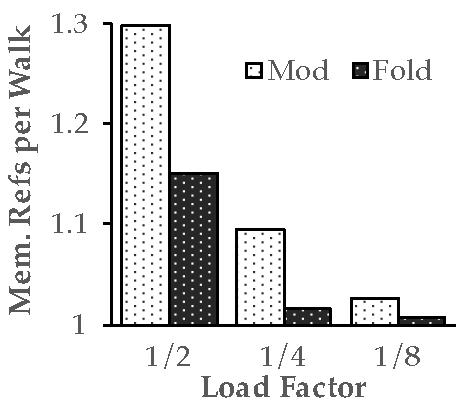
\includegraphics[width=0.45\columnwidth]{graphs/memrefs-bw.pdf}
   }
   \subfloat[\parbox{0.25\columnwidth}{Page walk latency normalized to DRAM latency.}]{
     \label{fig:pagewalklat}
     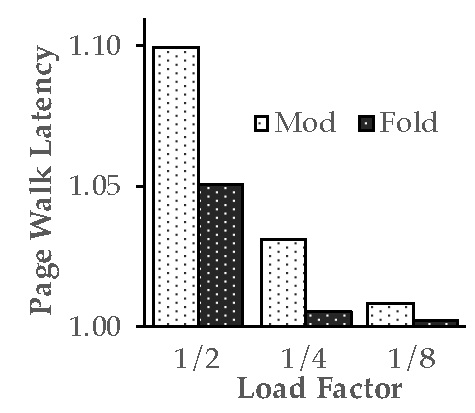
\includegraphics[width=0.45\columnwidth]{graphs/pagewalklat-bw.pdf}
   }
   \caption{Inverted page table performance.}
   \label{fig:IPT_perf_load_hash}
\end{figure}

Fig.~\ref{fig:pagewalklat} shows the page walk latency normalized to the latency of a single DRAM access. The page walk latency is within $1.005\times$ of a DRAM access. The reason the page walk latency does not directly correlate with the number of memory references per walk is that we use open addressing for resolving conflicts~\cite{yaniv:hash}. In open addressing, upon a collision, we probe the next entry in the inverted page table, rather than dereferencing a pointer to a new page table entry, exploiting the locality in the DRAM row buffer~\cite{qureshi:fundamental}, and thus reducing the latency overhead of collisions. Additionally, open addressing removes the pointer per page table entry required to resolve collisions. Each entry in our page table holds a 36-bit virtual page number (VPN), a 12-bit address space identifier (ASID), the 36-bit page frame number (PFN),\footnote{Note that we include the PFN and hence support synonyms.} and 12 bits for page flags, fitting in 16-byte entries. We assume 48-bit virtual and physical address. As we allocate four 16B entries for each 4KB page, due to the 1/4 load factor, the inverted page table consumes a modest $1.6\%$ of the physical memory.  

\subsection{TLB Hierarchy}
\label{sec:tlb}

Although a page walk usually introduces a single additional DRAM access within the memory partition, such accesses are still on the critical path. To minimize this overhead, we employ a TLB hierarchy within the memory-side MMUs to cache frequently used translations. Fig.~\ref{fig:tlb_hitratio} shows how the TLB hit ratio scales as the number of entries increases (more details on the methodology are found in Section~\ref{sec:methodology}). As our translation performance is less dependent on the TLB's hit ratio (due to fast page walks), we average the results across all workloads and scenarios. However, because the memory-side MMUs are shared across all processes in the system (in contrast to conventional MMUs which are bound to a single execution unit), we break down the average results across process counts. Although we expect few processes running concurrently on the MPU cluster,\footnote{A single process can run on an arbitrary number of MPUs.} we see that even with 8 different processes, a TLB with 64 entries, which is the usual size of a first-level TLB, achieves a hit ratio in excess of than $80\%$. Additionally, increasing the number of entries beyond 1024 gives diminishing results, which again matches the size of a conventional second-level TLB. Hence, a conventional two-level TLB hierarchy, a first level with 64 entries and a second level with 1024 is a sound approach. As each MMU integrates its own TLBs, its TLB content does not reflect accesses to others partitions and hence is robust across any memory chip and partition counts.

%All MPUs running in the same address space are a single process

\begin{figure}[t]
   \centering
   %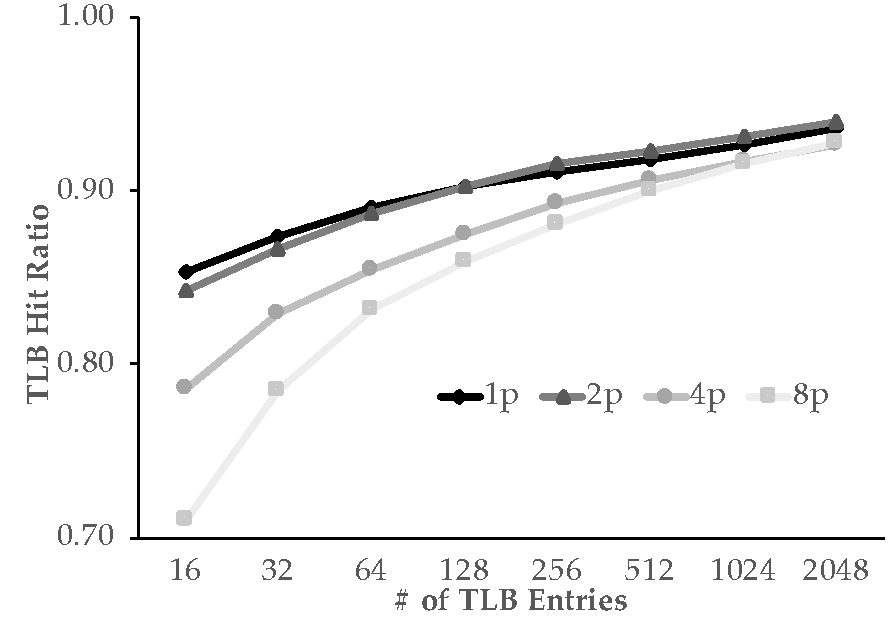
\includegraphics[width=0.8\columnwidth]{graphs/tlbhitratio-marker.pdf}
   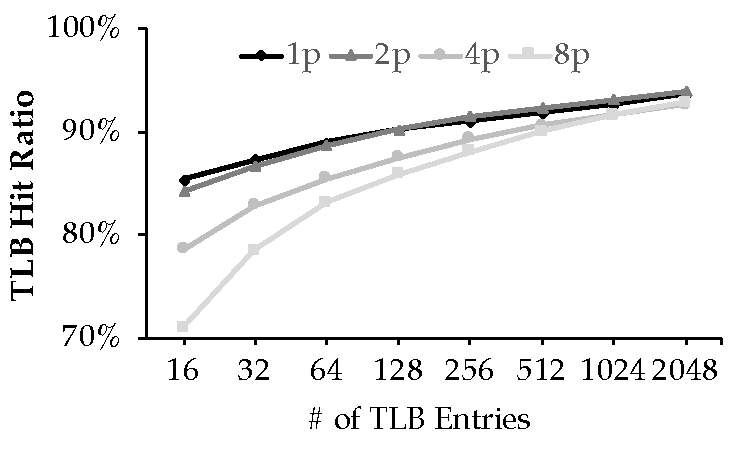
\includegraphics[width=0.8\columnwidth]{graphs/tlbmissratio.pdf}
   \caption{TLB hit ratio sensitivity analysis.}
   \label{fig:tlb_hitratio}
   
\end{figure}

\begin{figure}
\centering

 \subfloat[TLB hit operation.]{
  \label{fig:tlb_hit}
%  \includegraphics[width=.32\textwidth,clip,trim = 18mm 213mm 117mm 20mm]{figs/eps/sim-rread-lat.eps}}
   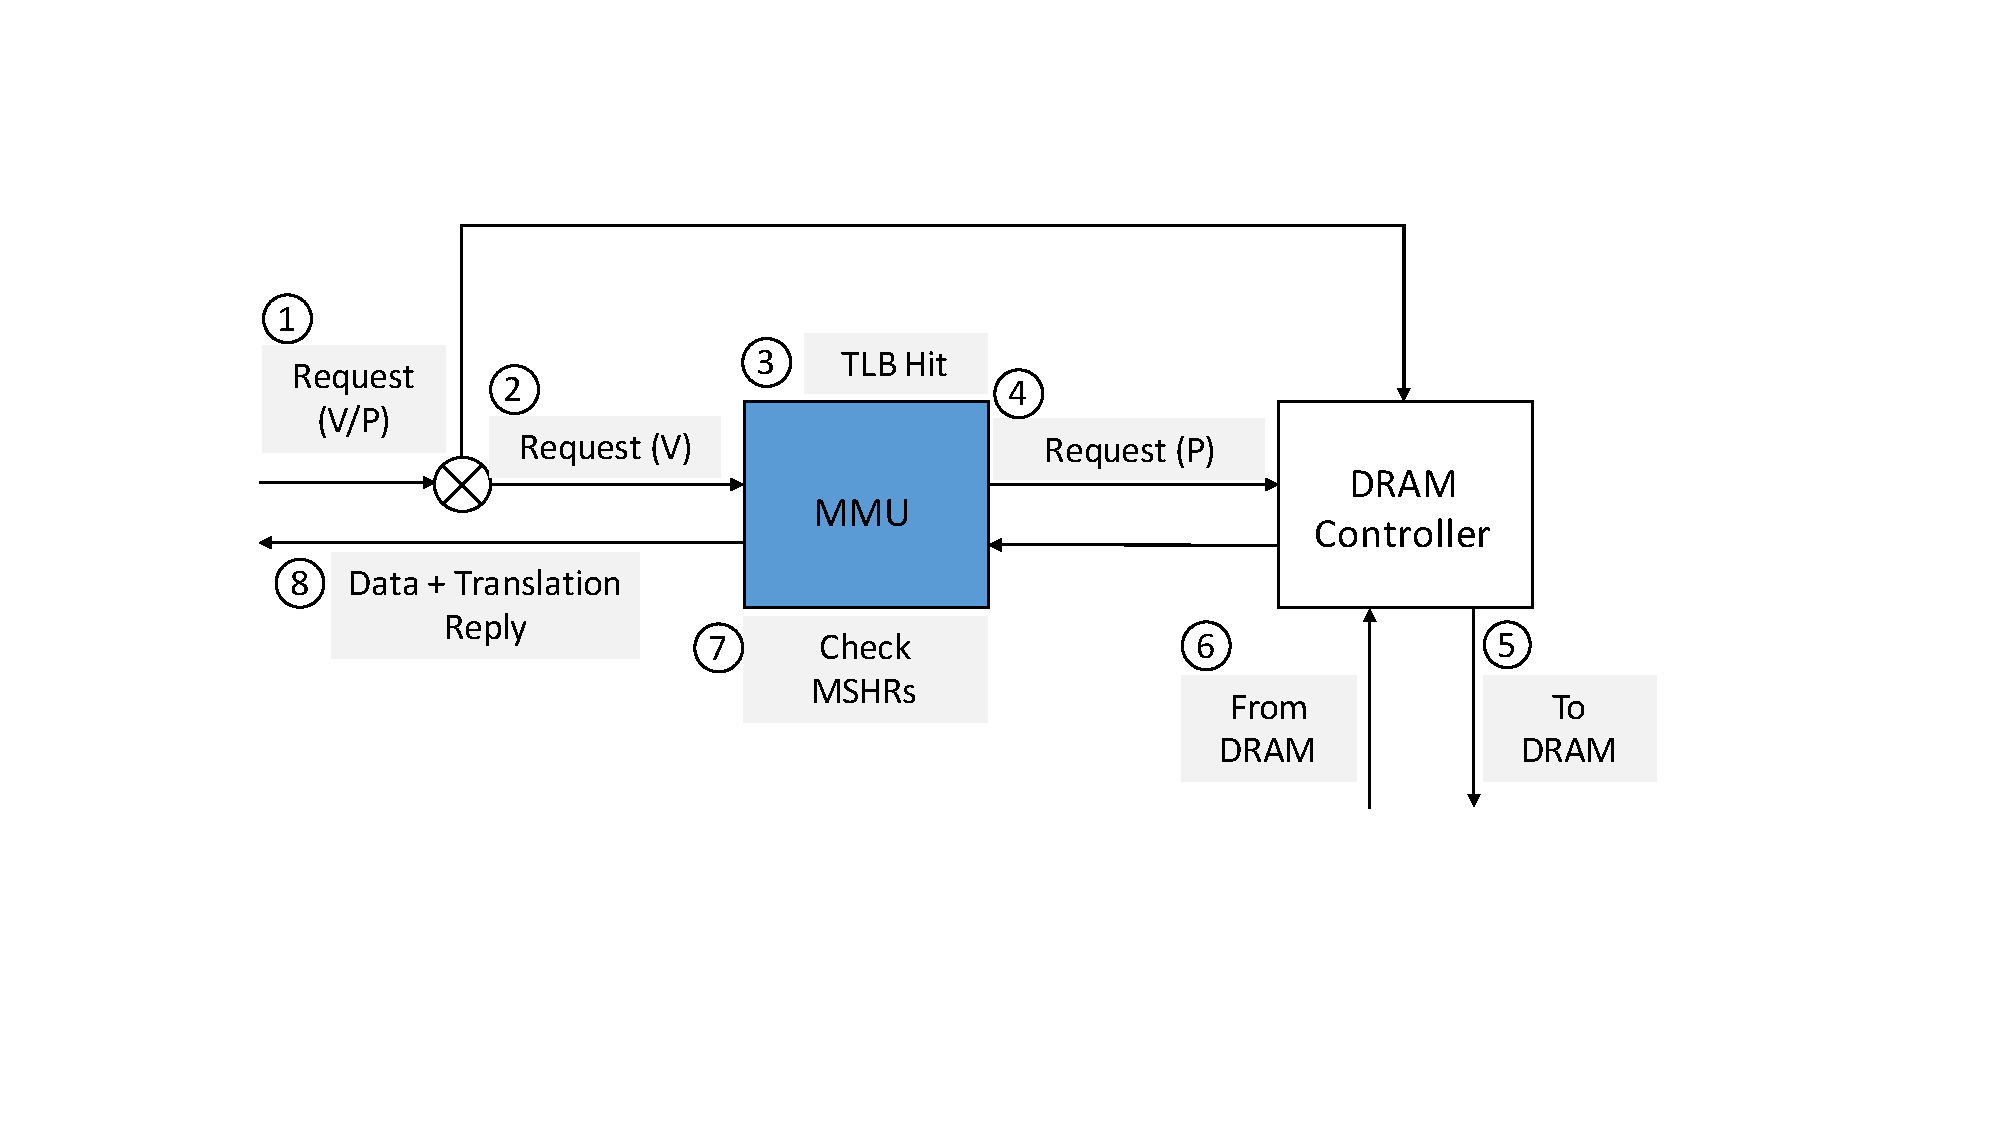
\includegraphics[clip,width=0.95\columnwidth]{figures/hit2.pdf}
   }
   
%  \hspace{.01in}

 \subfloat[TLB miss operation.]{
  \label{fig:tlb_miss}
%  \includegraphics[width=.32\textwidth,clip,trim = 18mm 213mm 115mm 20mm]{figs/eps/sim-rread-bw.eps}}
 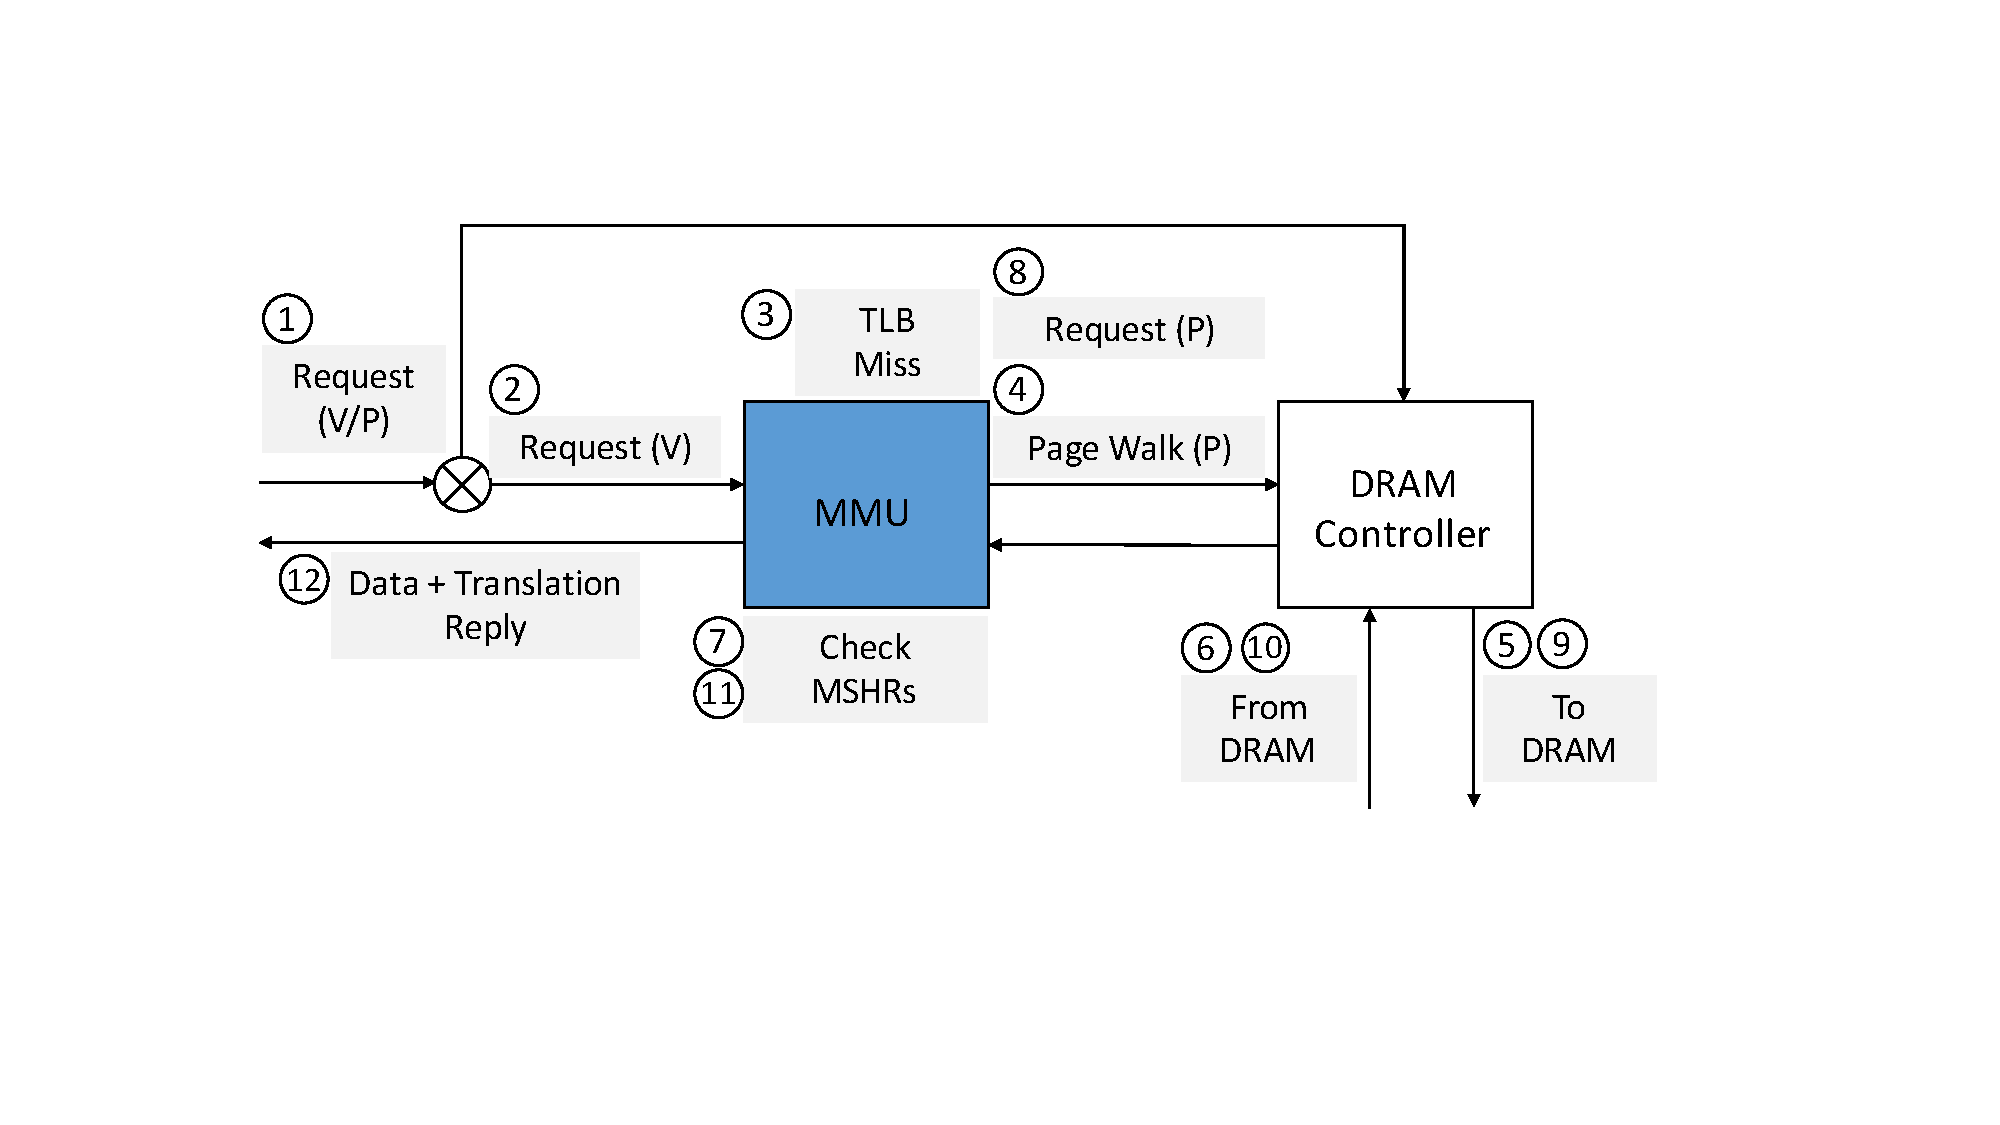
\includegraphics[clip,width=0.95\columnwidth]{figures/miss2.pdf}
 }

\caption{Operation flow of memory-side MMUs.
 \label{fig:tlb_ops}}
 
\end{figure}

\subsection{Putting Everything Together}
Now that we have defined the placement of the MMUs, the page table, and the TLB hierarchy, we provide a walkthrough of the memory-side MMU's operation in Fig.~\ref{fig:tlb_ops}.

In Fig.~\ref{fig:tlb_hit}, we look at the case where the TLBs in the memory-side MMU experience a hit. A request from an MPU arrives at the router of the target partition which forwards it to the MMU (1). A mux checks whether the message uses virtual or physical addresses (2). Memory requests that use physical addresses either come from CPU cores, DMAs, or MPUs that hit in their TLBs.\footnote{MPUs tag requests that use virtual addresses with a cookie.} In the case of physical addresses, the request is sent directly to the DRAM controller. In this example, the request uses virtual addresses, hence arriving at the MMU, and the TLB hierarchy is probed, resulting in a TLB hit (3). Note that the hit requires both the VPN and ASID bits (which are in the request) to match. The MMU then appends the offset bits to the PFN to generate the physical address, creates an MSHR entry tagged with the physical address, and sends a request to the DRAM controller (4). When the DRAM controller finds the address, it sends DRAM commands to fetch the appropriate cache block (5). When the reply comes back (6), the DRAM controller forwards the reply to the MMU, which checks the MSHRs for a match (7). Upon a match, the MMU sends the reply back to the MPU, containing both the data and translation (8).

In Fig.~\ref{fig:tlb_miss}, the memory-side MMU experiences a miss in its TLBs, triggering a page walk. A virtual request from an MPU arrives at the mux (1) and gets forwarded to the memory-side MMU (2). The MMU probes its TLB hierarchy, but the page table entry is not cached (3). The MMU generates the physical address of the page table entry by adding the output of the hash function on the request's virtual address to the base address of the inverted page table. The MMU then creates an MSHR entry tagged with this physical address and sends the request (for the page table entry) to the DRAM controller (4). When the DRAM controller finds the address, it sends DRAM commands to fetch the appropriate page table entry (5). When the reply comes back (6), the DRAM controller forwards the reply to the MMU. The MMU checks the MSHRs for a match (7). The matching MSHR entry indicates that it was a page walk, and hence the MMU generates the request for the actual cache block (8), and repeats the steps shown for the TLB hit operation: (9), (10), and (11). Last, the MMU sends the reply back to the MPU with the data and translation (12). 

Note that most of the functionality of the MSHRs in the MMU is performed by the request queues at the memory controller. We could extend the state of the queues and provide the same functionality. However, we avoid the complexity of extending the memory controller due to the modest hardware requirements for the MSHRs, 64 to 128 entries~\cite{lee:simultaneous} assuming worst-case overprovisioning. Additionally, to further reduce the already low bandwidth requirements of page walks (due to high TLB hit ratios), we indicate to the memory controller that the request for the page table entry is 16 bytes, instead of the conventional 64-byte requests. Existing memory controllers of 3D memories already support requests of different size~\cite{micron:hmc}.



\section{Operating System Support}
\label{sec:os}

\javier{Points to come across:

\begin{itemize}
  \item We need to remove the table. We need to write in a positive way that our changes are very simple and to prove it we managed to build a prototype. We need to explain the modifications with maybe pseudocode. Then, we can have a paragraph on the limitations of the prototype and talk about the memory-mapped files and explain what we would need to make it work, and why it is feasable. Maybe we can also talk about the COWs in SpryVM.
\end{itemize}

}

\begin{table*}[t]
%\small
\centering
\caption{Modifications required for OS mechanisms and policies to support spryVM.}
\label{tab:table_modifications}
\begin{tabular}{|c|l|}
\hline
Mechanism/Policy               & \multicolumn{1}{c|}{Modifications}                                                                                                                                                                                                                   \\ \hline
\multirow{2}{*}{Page Placement}   & \multirow{2}{*}{\begin{tabular}[c]{@{}l@{}}The policy needs to map a virtual page and its associated page frame to the same memory set. \\ FreeBSB implements a similar policy for cache sets~\cite{mckusick:design}, it should be extended to the memory.\end{tabular}} \\
                                  &                                                                                                                                                                                                                                                      \\ \hline
\multirow{2}{*}{Page Replacement} & \multirow{2}{*}{\begin{tabular}[c]{@{}l@{}} Global policies such as LRU or CLOCK do not require modifications as pages from all sets are\\eviction candidates. For dramatically low-memory cases, evictions prioritized by set are interesting.\end{tabular}} \\
                                  &                                                                 \\ \hline
\multirow{2}{*}{Page Tables} & \multirow{2}{*}{\begin{tabular}[c]{@{}l@{}}The OS needs to set up and manage two page tables: native and spryVM. Linux HMM patch deals \\on setting up and maintaining multiple page tables consistent upon any changes to the mappings~\cite{glisse:hmm}.\end{tabular}}                  \\ 
                                  &                                                                                                                                                                                                                                                      \\ \hline
Page Cache                        & \begin{tabular}[c]{@{}l@{}}Page allocation due to reads \& writes to block devices or swap files do not require modifications. A\\ page allocated of a memory-mapped file requires virtual and physical pages mapping to the same set.\end{tabular}                  \\ \hline
\multirow{2}{*}{Synonyms}         & \multirow{2}{*}{\begin{tabular}[c]{@{}l@{}}All synonyms of a virtual page need to map to the same memory set. Prior systems included this policy\\ for cache sets~\cite{cheng:virtual}, it should be extended to memory. COW works as is as virtual pages are identical.\end{tabular}} \\
                                  &                                                                                                                                                                                                                                                      \\ \hline
\end{tabular}
\end{table*}

\begin{table*}[t]
\centering
%\small
\caption{Operating system overheads for spryVM support.}
\label{tab:table_overheads}
\begin{tabular}{|c|l|}
\hline
Mechanism/Policy               & \multicolumn{1}{c|}{Overheads}                                                                                                                                                                                                                   \\ \hline
\multirow{2}{*}{Page Placement}   & \multirow{2}{*}{\begin{tabular}[c]{@{}l@{}}Though a few ways per process evenly distributes pages across memory sets for our workloads, there\\ could be cases where an excess of page faults arises due to underutilized memory sets.\end{tabular}} \\
                                  &                                                                                                                                                                                                                                                      \\ \hline
\multirow{2}{*}{Page Replacement} & \multirow{2}{*}{\begin{tabular}[c]{@{}l@{}} If evictions prioritized by set is implemented, page reclamation is more costly as traversing the\\ inactive list of pages needs now to consider only pages of a particular memory set.\end{tabular}} \\
                                  &                                                                 \\ \hline
\multirow{2}{*}{Page Tables} & \multirow{2}{*}{\begin{tabular}[c]{@{}l@{}}TLB shootdowns and page table updates~\cite{black:translation} need to span spryVM's TLBs and page table. Though\\ we expect a low overhead as a virtual page maps to one set, and hence one MMU \& page table slice.\end{tabular}}                  \\ 
                                  &                                                                                                                                                                                                                                                      \\ \hline
Page Cache                        & \begin{tabular}[c]{@{}l@{}}Having different allocation policies in the page cache complicates the design and adds overhead.\\ Alternatively, we could use one policy for all pages: virtual \& physical pages map to the same set. \end{tabular}                  \\ \hline
\multirow{2}{*}{Synonyms}         & \multirow{2}{*}{\begin{tabular}[c]{@{}l@{}} Communication between processes through shared memory employs the page cache layer, and hence\\ the overheads would be similar to the previous case: an increase in code complexity in the page cache.\\ \end{tabular}} \\
                                  &                                                                                                                                                                                                                                                      \\ \hline
\end{tabular}
\end{table*}

SpryVM requires a number of operating system (OS) modifications. The OS must assign page frames to virtual pages so that both pages map to the same memory set. Furthermore, the OS must create and manage spryVM's inverted page table, and synchronize it with the native page table. Although end-to-end performance evaluation requires a full implementation of spryVM in a modern OS (e.g., Linux, FreeBSD), like prior work which require OS changes \cite{talluri:surpassing, talluri:tradeoffs, talluri:pagetable}, we note that such implementation is a multi-man-year project. Consequently, like those studies, we instead inspect an open-source OS (i.e., Linux) and qualitatively discuss our proposed modifications.  

Fortunately, our two main modifications (i.e., memory-set matching and managing multiple page tables) are currently implemented in modern OS's. For instance, FreeBSD implements page coloring to avoid consecutive virtual pages mapping to the same cache set. FreeBSB does this with a free list of pages per cache set~\cite{mckusick:design}, guaranteeing that two consecutive virtual pages map to different cache sets. We can similarly extend the page placement policy to make both the VPN and PFN map to the same memory set. Further, the Linux Heterogeneous Memory Management (HMM) patch sets up multiple page tables and maintains the consistency~\cite{glisse:hmm}. We can leverage the lessons learned from these patches.

Table~\ref{tab:table_modifications} and Table~\ref{tab:table_overheads} shed more light on the OS changes and the potential overheads respectively. Although set associative VM is beneficial for a wide range of workloads, there might be cases for which full associative VM is required. Hence, we envision spryVM to be an optional optimization (i.e., a process, set of processes, or the whole system can fall back to the conventional translation). This is conceptually similar to the way OSes support superpages, for which large portions of the OS required modifications along with their associated overheads with respect to supporting a single page size~\cite{talluri:surpassing, navarro:practical, kwon:coordinated}. Analogously, when super pages are not beneficial or impossible to generate, processes fall back to base pages. 
 
 %MIPS OS searched the free list of pages to find a page frame that maps to the same first-level cache set as the virtual page (i.e., page coloring)~\cite{taylor:tlb}.

%We could basically say that what we're doing uses known techniques to leverage a novel observation (set-associativity). 

%As a specific example, take the fact that we're setting up multiple page tables. Well, the latest Linux HMM patch does exactly this, so Linux developers already tackled all the challenges of syncing up two page tables. We could basically say that what we're doing uses known techniques to leverage a novel observation (set-associativity). 

%RMM requires modest operating system (OS) modifications.The OS must create and manage range table entries in softwareand coordinate them with the page table. We modify the OS to increase the size of ranges with an eager paging allocation mechanism. We prototype these changes in Linux, but thedesign is applicable to other OSes.

%The really big concern that we have to hit out of the park is the last MICRO reviewer's concern of OS changes. I agree that fully implementing this in Linux/FreeBSD/sv6/etc. would instill more confidence that spryVM/spryVM works effectively. However, I also don't think that this is a reasonable bar for an academic paper. To address this, my first instinct is to go the following route:

\subsection{Support spryVM with NUMA page allocation policy}
In practice,  mapping only a subset of physical pages to given virtual addresses is very similar to a scenario existing in NUMA systems — binding the memory of a process to a specific NUMA nodes. With NUMA memory bind policy (i.e. \textit{membind}), a process is only able to get physical pages coming from the NUMA node assigned by the policy, where, with spryVM, each subset of a process’s virtual address space can be seen as being bound to a certain NUMA node. As a result, to implement spryVM in operating systems, we are able to reuse most of existing NUMA-related code. In a spryVM system, each memory set can be treated as a NUMA node and all processes have membind as their default memory allocation policy. Whenever a page fault happens, during the process of physical page allocation, the operating system calculates the corresponding NUMA node id from the faulting virtual address with our hash function, then obtains a free page from that NUMA node and finishes the page fault process. Taking Linux as an example, \verb|alloc_pages_vma()| is the entry point of each user space  page allocation, thus, we simply calculate a memory set index (stored in a NUMA node mask variable) out of the faulting address, derive the corresponding zone list, and pass them to the page allocation function — \verb|__alloc_pages_nodemask()|. Linux is able to handle the rest of page fault work without any problem.

For inverted page tables, x86 systems do not have them, but they are very commonly used in IBM Power systems as hashed page tables. Thus, we follow the same operation model as hashed page tables in IBM Power systems: reserving memory for each inverted page table in individual NUMA node and inserting/invalidating/updating inverted page table entries whenever CPU page tables change in the same hook functions (e.g. \verb|update_mmu_cache()|). To guarantee the translation information is coherent between CPUs and accelerators, each inverted page table entry has a valid bit, which is atomically accessed by both CPUs (for inverted page table modification) and accelerators (for reading). Alternatively, if accelerators, e.g. GPUs, want to maintain their own page tables instead of using the inverted page table, additional hook functions, like  \verb|mmu_notifier| mechanism in Linux, could be used to keep the page tables of accelerators coherent with CPU page tables.

Both modifications are very simple and not intrusive to operating systems. We only add around 200 lines of code in Linux to achieve the required functionality for spryVM. 

\begin{algorithm}
  \caption{Memory set indexing algorithm}\label{alg:index}
  \begin{algorithmic}[1]
    \Procedure{alloc\_pages\_vma}{\textbf{addr\_t} vaddr}
    \State $\textit{mem\_set\_id} \gets \verb|MEM_SET_INDEX_HASH|(\mbox{vaddr})$
    \State $\textit{page} \gets \verb|alloc_pages_node|(\mbox{vaddr}, \mbox{mem\_set\_id})$
    \State \textbf{return} \textit{page}
    \EndProcedure
  \end{algorithmic}
\end{algorithm}
\section{Experimental Methodology}
\label{sec:methodology}

\begin{table}
        \begin{center}
                \caption{Server Workload description.}
                \scalebox{0.7}
                \small
                \vspace{0.01in}
                \label{table:workload}
                \renewcommand{\arraystretch}{1.0}
                {\scriptsize
                        \begin{tabular}{ l  l }
                                \toprule
                                {\bf Workload}                  & {\bf Description}  \\
                                \toprule
                                \multirow{1}{*}{Cassandra}      &  NoSQL data store running Yahoo's YCSB. \\
                                \cmidrule{2-2}
                                \multirow{1}{*}{Memcached}      & Cache store running Twitter-like workload~\cite{lim:thin}. \\
                                \cmidrule{2-2}
                                \multirow{1}{*}{TPC-H}          & TPC-H on MonetDB column store (Q1-Q21). \\
                                \cmidrule{2-2}
                                \multirow{1}{*}{TPC-DS}         & TPC-DS on MonetDB column store (Queries of~\cite{kocberber:meet}). \\
                                \cmidrule{2-2}
                                \multirow{1}{*}{MySQL}          & SQL DBMS running Facebook's LinkBench~\cite{facebook:linkbench}. \\
                                \cmidrule{2-2}
                                \multirow{1}{*}{RocksDB}        &  Store engine running Facebook benchmarks~\cite{facebook:rocksdb}. \\ %a canonical uniform request distribution. \\

                                \bottomrule
                        \end{tabular}
                } %small
        \end{center}
        \vspace{-0.1in}
\end{table}

Like most recent work on VM~\cite{basu:efficient, pham:increasing, pham:colt, bhattacharjee:large-reach, barr:spectlb, papadopoulou:prediction-based, saulsbury:recently-based}, we use a combination of real-hardware measurements, trace-driven functional simulation, analytical models, and linux kernel prototypes.

\subsection{Workloads}

To study the impact of associativity on general-purpose software, we use a suite of popular server workloads, shown in Table~\ref{table:workload}, in a variety of setups. First, we use them to study the very limits of reducing associativity using a 3C page fault model and Pin traces. For practical reasons these workloads are tuned to fit in 8GB memory for this experiment. Then we study the behavior of the server workloads on real hardware with our modified linux kernel (v4.10) with set-associative memory (which we plan to open-source), using more realistic dataset sizes (16-32GB), in both in-memory and out-of-memory setups.

To study the TLB behavior at very large datasets (128GB), we use  data traversal applications present in the ASCYLIB~\cite{david:asynchronized} suite, which contains state-of-the-art implementations of hash tables, extarnal and internal binary trees, and skip lists, which are the core of many of the server workloads, such as Memcached and RocksDB. We choose these workloads because of their minimal data locality and instruction-level parallelism, and the fact that they are stressing conventional general-purpose CPU architectures and hence favor custom hardware~\cite{ haria:devirtualizing, picorel:near-memory, kocberber:meet, hsieh:accelerating}. Similar to prior work~\cite{picorel:near-memory}, we present the results for four representative implementations for space reasons. 

%: Java Hash Table (Hash Table), Fraser Skip List (Skip List), Howley Binary Search Tree (BST Internal), and Natarajan Binary Search Tree (BST External).

%Furthermore, following the premises of a unified VM and enabling "pointer-is-a-pointer" semantics, it is not expected that accelerators will run an end-to-end workload in isolation. In contrast, the expected model is to offload certain parts of the CPU's execution which are more efficiently executed on the accelerators. Although the offloading mechanism is out of the scope of this paper, we decided to stress the notion of associativity in VM with a set of popular server workload, shown in Table~\ref{table:workload}. The reason is that these workloads stress the VM mechanism, with large memory requirements, often allocation and de-allocation of memory, and overly fragmented virtual memory layouts~\cite{picorel:near-memory}. Moreover, the evaluated data structure traversals are in fact the core of many of the server workloads, such as Memcached's hash table and RocksDB' skip list data structures.

\subsection{TLB studies}
To study the impact of memory size on  TLB performance (Figure~\ref{fig:pagewalks}), we perform measurements on real hardware using the \textit{perf} tool during a 10min execution window. To study the TLB capacity requirements of different designs, we collect memory traces for 128GB datasets using Pin~\cite{luk:pin}, with each trace containing 1B instructions, which is more than enough for the TLB sensitivity experiments up to a few thousand entries. We use the traces to probe a set-associative TLB structure while varying its size and organization, after validating the baseline TLB model against the measurements on real hardware. 

\subsection{Limits of Associativity Reduction}

%As modern systems place no restrictions on the virtual-to-physical mapping, address translation is on the critical path of every memory access. To break translation and data path serialization, prior work proposes to eliminate associativity and enforce a direct mapping between virtual pages and page frames~\cite{picorel:near-memory, haria:devirtualizing}. As every virtual page can only map to one single location, translation and data paths are independent and can proceed in parallel.

As our approach intends to find a middle-ground between fully associative (i.e., conventional translation) and direct mapping~\cite{picorel:near-memory, haria:devirtualizing}, we aim to fill the research void of what is the level of associativity needed. Interestingly enough, there exists no study on VM associativity, unlike caches, which are similar in some organizational aspects and for which such a study has existed for three decades~\cite{hill:aspects}. To study the VM associativity, we employ the well-established 3C model---initially developed for caches~\cite{hill:aspects}. In this context, associativity means the number of possible locations (page frames) a given virtual page can map to. This model classifies misses (i.e., page faults) into three categories: conflict misses (when too many active pages map to a fraction of the sets), capacity misses (due to limited memory size), and compulsory misses (upon the first access to a page). 

%One potential way to break translation-memory access serialization is to completely eliminate associativity and enforce a direct mapping between virtual pages and page frames. Since a virtual page can now only map to a single page frame, address translation and data fetch are independent and can proceed in parallel. Conventional wisdom dictates that direct mapping creates an excess of page faults, due to conflicts from multiple virtual pages mapping to the same page frame. However, this is merely intuition, as there exists no study on VM associativity, unlike caches, which are similar in some organizational aspects and for which such a study has existed for three decades~\cite{hill:aspects}. 


%To fill this research void, we employ the 3C model---initially developed for caches~\cite{hill:aspects}---to study VM associativity. In this context, associativity means the number of possible locations (page frames) a given virtual page can map to. This model classifies misses (i.e., page faults) into three categories: conflict misses (when too many active pages map to a fraction of the sets), capacity misses (due to limited memory size), and compulsory misses (upon the first access to a page). 

%To simulate real-world scenarios, we select a set of representative server workloads, summarized in Table~\ref{table:workload}. We include two cloud workloads from CloudSuite~\cite{ferdman:clearing}, Cassandra and Memcached, an online transaction processing (OLTP) workload~\cite{facebook:linkbench}, MySQL, two online analytical processing (OLAP) workloads~\cite{boncz:breaking}, TPC-H and TPC-DS, and a widely-used storage system workload~\cite{dong:optimizing}, RocksDB. We collect long memory traces of several 10s of billions of instructions of the server workloads using Pin~\cite{luk:pin}. We extract the virtual address and address space identifier (ASID) of each memory reference and use it to probe a set-associative memory structure, varying the associativity to observe and classify the misses. A detailed description of our methodology is found in Section~\ref{sec:methodology}.

%\subsection{Single-Process In-Memory}

%Fig.~\ref{fig:miss_ratio} shows results for three single-process
%workloads: Memcached, RocksDB, and Cassandra. The y-axis breaks down
%the total misses into the three distinct miss classes. Each category
%on the x-axis corresponds to the ratio between the size of the
%physical memory and the size of the application's working set. For
%example, $8\times$ indicates that the memory is eight times larger
%than the application's working set. Similarly, $1/2\times$ means that
%the application's working set is twice the size of the memory. We
%collapse results for $8\times$ to $1\times$ because they are similar
%and visually identical; each case represents a fully in-memory
%scenario. Furthermore, within each working set category, the x-axis
%sweeps through different VM associativities, from direct-mapped to
%32-way associative.


We collect memory traces using Pin~\cite{luk:pin}. For workloads with fine-grained operations (i.e., Memcached, RocksDB, MySQL, and Cassandra), the traces contain the same number of instructions as the application executes in 60 seconds without Pin. For analytics workloads (i.e., TPC-H \& TPC-DS), we instrument the entire execution. We extract the ASID bits and virtual address of each memory access, concatenate both~\cite{basu:reducing, yoon:revisiting},  and use it to probe a set-associative memory structure. For the associativity experiments, we tune all the workloads to have a resident set size (RSS) of 8GB. In other words, the allocated physical memory for all the processes of a given workload is 8GB. For single-process runs, a single process has an RSS of 8GBs. For two-process runs, each of the processes has an RSS of 4GB. The same scaling applies for the runs with four and eight processes. To vary the memory size to working set size ratio, we vary the size of the set-associative memory structure. 

%We use the same traces for the page table experiments of Section~\ref{sec:pagetable} and feed them into our inverted page table modeling tool. For the TLB experiments in Section~\ref{sec:tlb} and the performance experiments in Section~\ref{sec:evaluation}, we tune the workloads to employ working sets of size 32GB and 64GB, depending on the size of the network. We use 32GB and 64GB for 4- and 8-chip, and 16-chip configurations respectively.

We collect the traces on a dual-socket server CPU (Intel Xeon E5-2680 v3) with $256$GB of memory, using the Linux 3.10 kernel and Google's TCMalloc~\cite{google:tcmalloc}. Address space randomization (ASLR) is enabled in all experiments.

\subsection{Performance}


Full-system simulation for TLB misses and page faults is not practical, as these events occur less frequently than other micro-architectural events (e.g., branch mispredictions). Hence, we resort to the CPI models often used in VM research~\cite{papadopoulou:prediction-based, saulsbury:recently-based, bhattacharjee:shared} to sketch the performance gains. These prior studies report performance as the reduction in the translation-related cycles per instruction. As CPI components are additive, this metric is valid irrespective of the workload's baseline CPI. We further strengthen this methodology by studying the CPI savings on all memory operations, not only on translation (as we overlap translation and data fetch operations). Our model thus captures both the translation and data fetch cycles, which together constitute the largest fraction of the total CPI in data structure traversals~\cite{picorel:near-memory}. The CPI is measured by applying fixed penalties to the TLB miss rates obtained with the PIN traces. 


%\section{Evaluation}
\label{sec:evaluation}

\begin{figure*}
	\centering
	\subfloat[Memcached --- 1 Process]{
		\label{fig:memcached_1p}
		%  \includegraphics[width=.32\textwidth,clip,trim = 18mm 213mm 117mm 20mm]{figs/eps/sim-rread-lat.eps}}
		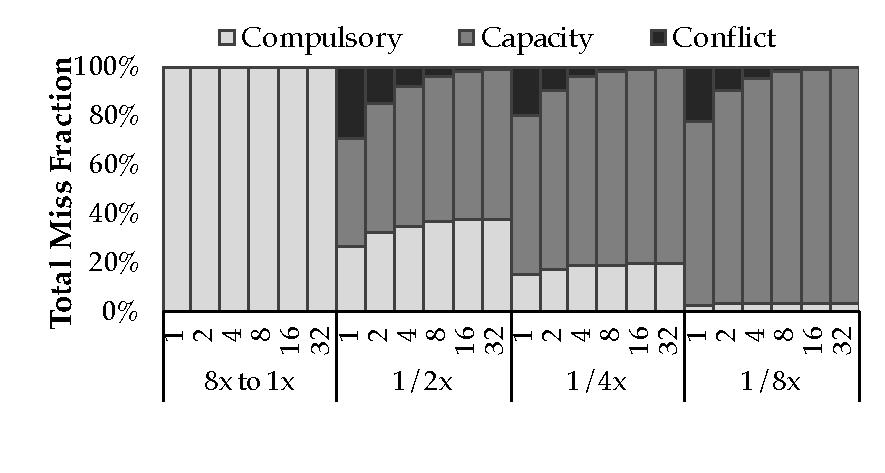
\includegraphics[width=.365\textwidth,clip]{graphs/memcached_assoc_1p-bw.pdf}}
	%  \hspace{.01in}
	\subfloat[RocksDB --- 1 Process]{
		\label{fig:rocksdb_1p}
		%  \includegraphics[width=.32\textwidth,clip,trim = 18mm 213mm 115mm 20mm]{figs/eps/sim-rread-bw.eps}}
		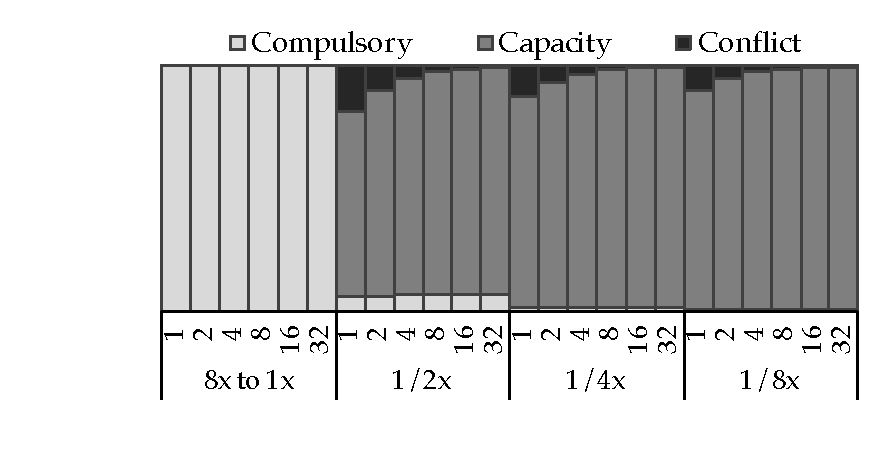
\includegraphics[width=.31\textwidth,clip]{graphs/rocksdb_assoc_1p-bw.pdf}}
	%   \hspace{.01in}
	\subfloat[Cassandra --- 1 Process]{
		\label{fig:cassandra_1p}
		%  \includegraphics[width=.32\textwidth,clip,trim = 28mm 217mm 115mm 20mm]{figs/eps/emu-rread-lat_cropped.eps}}
		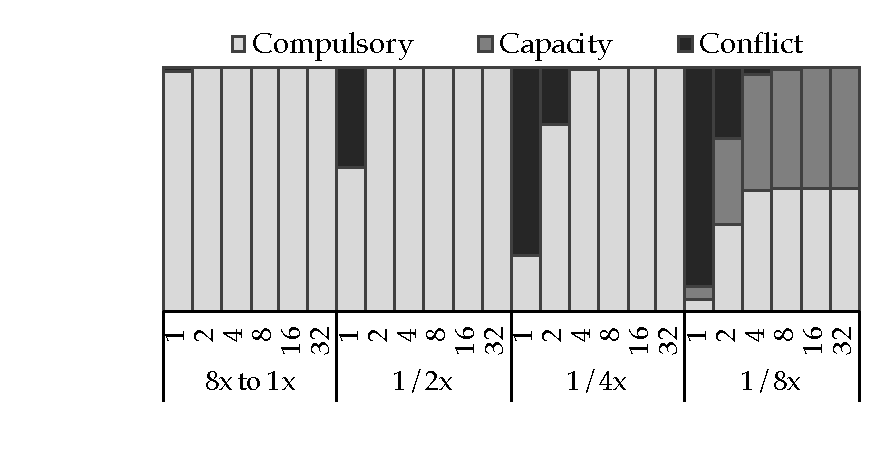
\includegraphics[width=.31\textwidth,clip]{graphs/cassandra_assoc_1p-bw.pdf}}
	\caption{Overall miss ratio broken down into compulsory, capacity, and conflict misses.
		\label{fig:miss_ratio}}
\end{figure*}

%%%%%%%%%%% Table: Methodology %%%%%%%%%%%
\begin{table}
	\begin{center}
		\caption{Workload description.}
		\scalebox{0.7}
		\small
		\vspace{0.01in}
		\label{table:workload}
		\renewcommand{\arraystretch}{1.0}
		{\scriptsize
			\begin{tabular}{ l  l }
				%\hline
				\toprule
				{\bf Workload}                  & {\bf Description}  \\
				%\hline
				%\hline
				\toprule
				\multirow{1}{*}{Cassandra}                       &  NoSQL data store running Yahoo's YCSB. \\
				%\hline
				\cmidrule{2-2}
				\multirow{1}{*}{Memcached}                      & Cache store running Twitter-like workload~\cite{lim:thin}. \\
				%\hline
				\cmidrule{2-2}
				%\multirow{2}{*}{Core Types}    & In-order (Cortex A8-like): 2-wide \\
				%		                               &  OoO (Xeon-like): 4-wide, 128-entry ROB \\
				%\hline
				\multirow{1}{*}{TPC-H}	& TPC-H on MonetDB column store (Q1-Q21). \\
				\cmidrule{2-2}
				\multirow{1}{*}{TPC-DS}	& TPC-DS on MonetDB column store (Queries of~\cite{kocberber:meet}). \\
				\cmidrule{2-2}
				%\multirow{2}{*}{L1-I/D Caches}	&	32KB, split, 2 ports, 64B blocks, 10 MSHRs, \\
				%							& 2-cycle load-to-use latency \\
				\multirow{1}{*}{MySQL} 			& SQL DBMS running Facebook's LinkBench~\cite{facebook:linkbench}. \\
				%\hline
				\cmidrule{2-2}
				\multirow{1}{*}{RocksDB}                             &  Store engine running Facebook benchmarks~\cite{facebook:rocksdb}. \\ %a canonical uniform request distribution. \\
				%\hline
				
				\bottomrule
				%\hline
			\end{tabular}
		} %small
	\end{center}
	\vspace{-0.1in}
\end{table}
%%%%%%%%%%% END Table: Methodology %%%%%%%%%%%%

\begin{figure*}[t]
	\centering
	\subfloat[Memcached --- 2 Processes]{
		\label{fig:memcached_2p_assoc}
		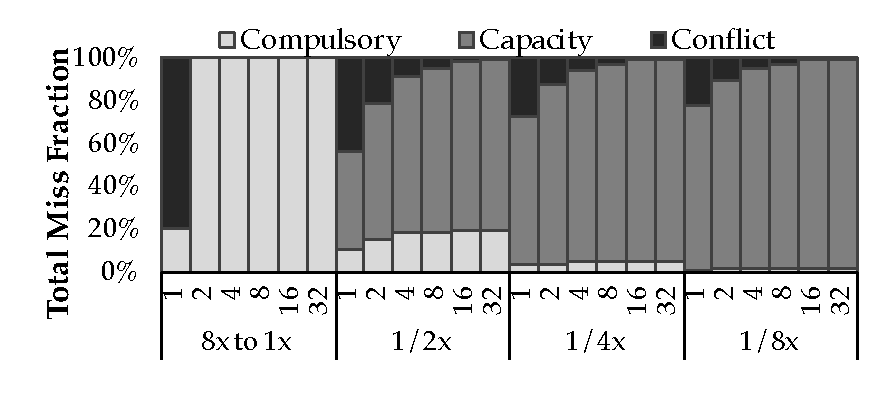
\includegraphics[width=.36\textwidth,clip]{graphs/memcached_assoc_2p-bw.pdf}}
	\subfloat[Memcached --- 4 Processes]{
		\label{fig:memcached_4p_assoc}
		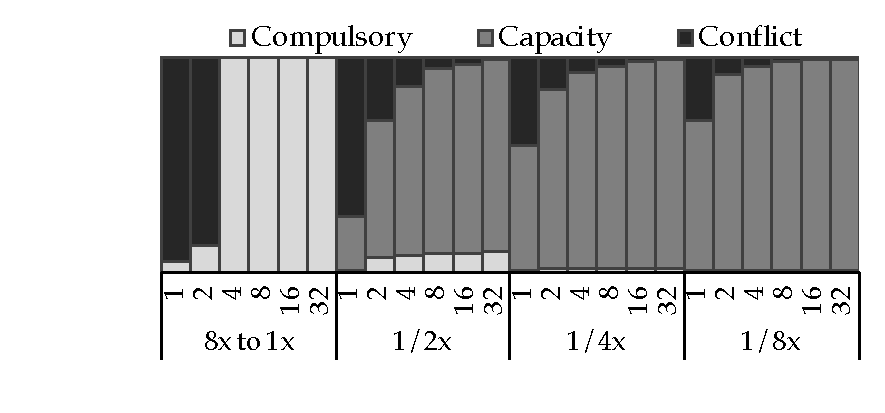
\includegraphics[width=.31\textwidth,clip]{graphs/memcached_assoc_4p-bw.pdf}}
	\subfloat[Memcached --- 8 Processes]{
		\label{fig:memcached_8p}
		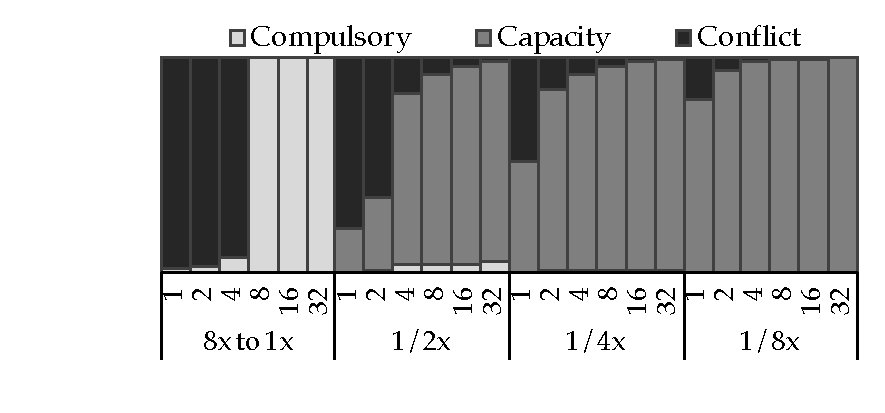
\includegraphics[width=.31\textwidth,clip]{graphs/memcached_assoc_8p-bw.pdf}}
	\hspace{.01in}
	\subfloat[RocksDB --- 2 Processes]{
		\label{fig:rocksdb_2p}
		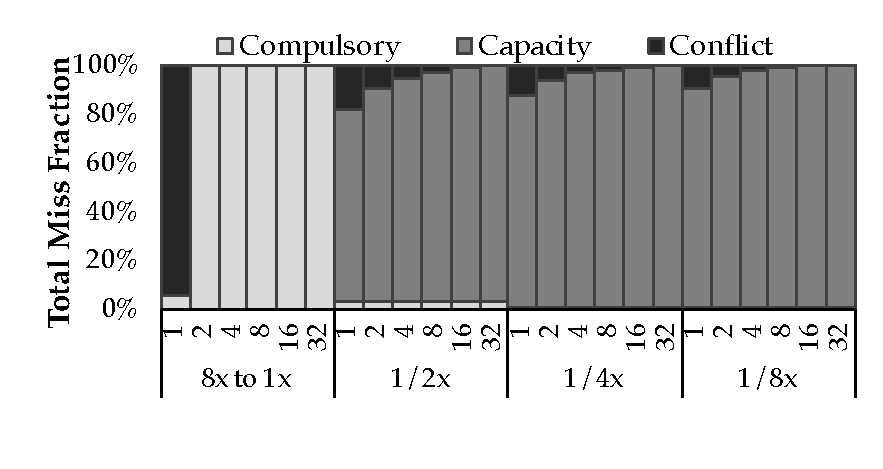
\includegraphics[width=.36\textwidth,clip]{graphs/rocksdb_assoc_2p-bw.pdf}}
	\subfloat[RocksDB --- 4 Processes]{
		\label{fig:rocksdb_4p}
		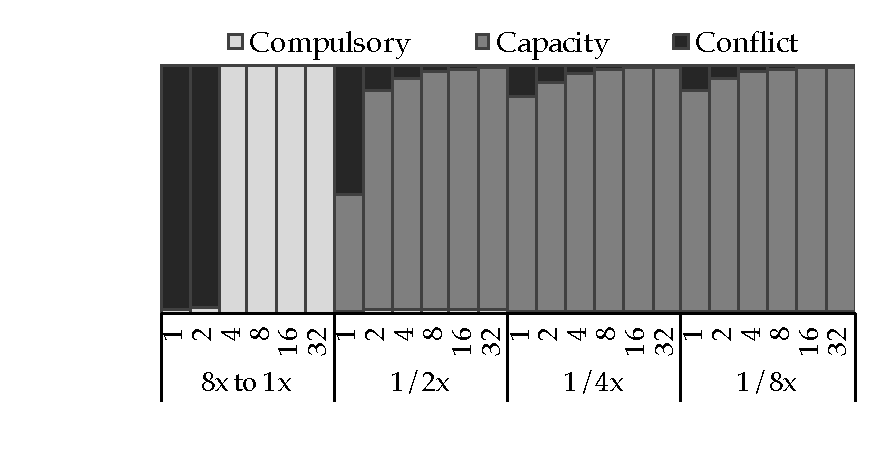
\includegraphics[width=.305\textwidth,clip]{graphs/rocksdb_assoc_4p-bw.pdf}}
	\subfloat[RocksDB --- 8 Processes]{
		\label{fig:rocksdb_8p}
		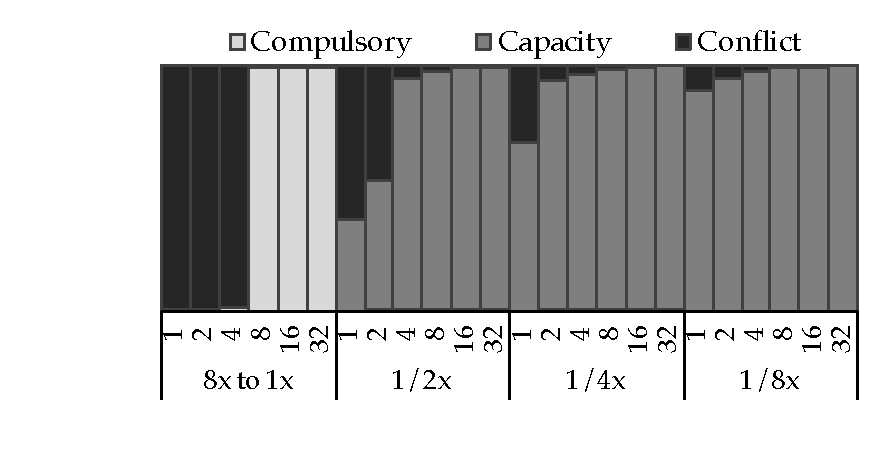
\includegraphics[width=.31\textwidth,clip]{graphs/rocksdb_assoc_8p-bw.pdf}}
	\hspace{.01in}
	\subfloat[Cassandra --- 2 Processes]{
		\label{fig:cassandra_2p}
		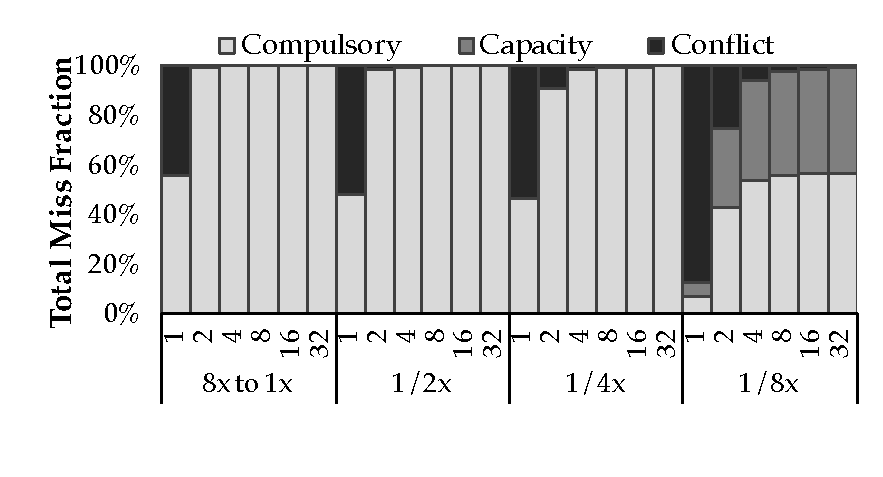
\includegraphics[width=.355\textwidth,clip]{graphs/cassandra_assoc_2p-bw.pdf}}
	\subfloat[Cassandra --- 4 Processes]{
		\label{fig:cassandra_4p}
		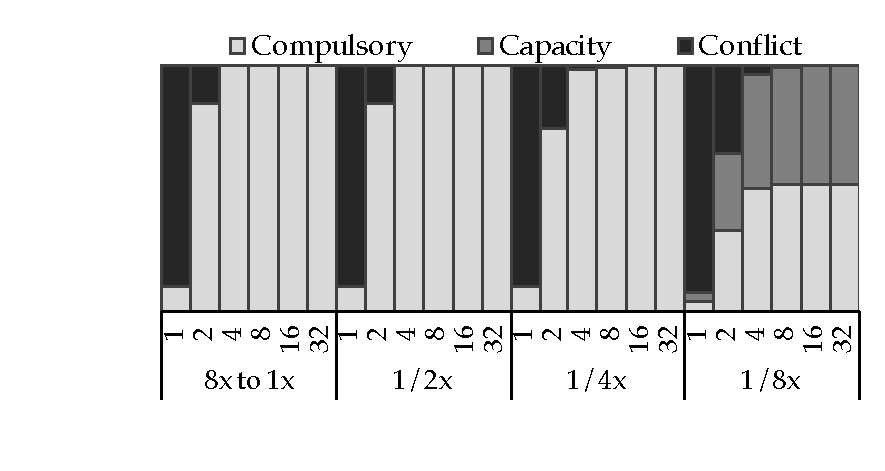
\includegraphics[width=.31\textwidth,clip]{graphs/cassandra_assoc_4p-bw.pdf}}
	\subfloat[Cassandra --- 8 Processes]{
		\label{fig:cassandra_8p}
		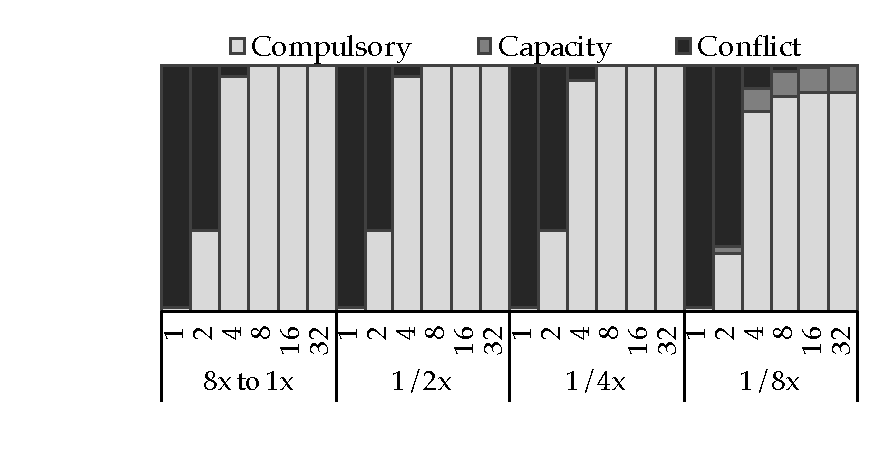
\includegraphics[width=.31\textwidth,clip]{graphs/cassandra_assoc_8p-bw.pdf}}
	
	
	\caption{Overall miss ratio broken down into compulsory, capacity, and conflict misses.
		\label{fig:miss_ratio_procs}}
\end{figure*}


%\javier{Points to come across:

%\begin{itemize}
%  \item Set-associativity doesn't increase page faults: 3C model %+ Memcached and RocksDB on real HW
%  \item TLB miss rate vs. working set for microkernels (hash %table, skip list, bst internal, bst external)
%  \item TLB miss penalty vs. working set (or sockets)
%  \item Fragmentation
%  \item $IPC =IPC_base + Penalty_tlb + Penalty_page_faults$
%\end{itemize}
%
%}


%\begin{figure*}[!h]
%\centering
% 
%  \subfloat[In-memory scenario.]{
%  \label{fig:speedup_memory_in}
%
%   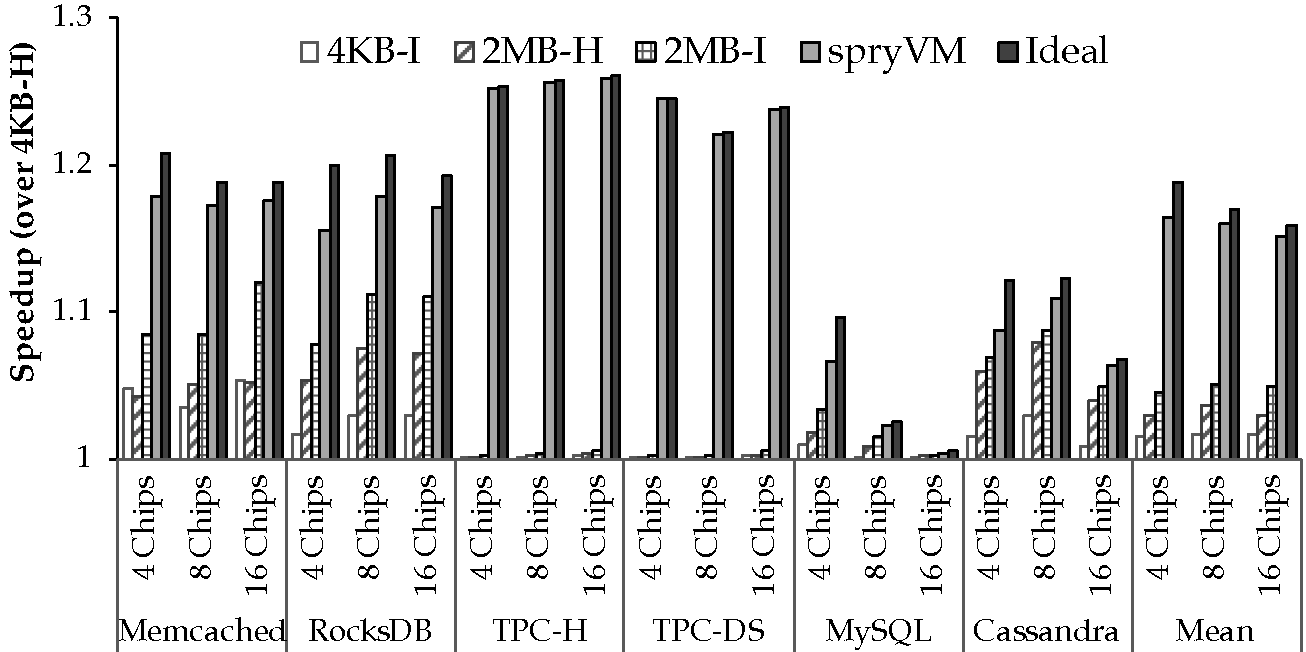
\includegraphics[width=0.48\textwidth,clip]{graphs/speedup_inmemory.pdf}
%   }
%
%
%  \subfloat[Out-of-memory scenario.]{
%  \label{fig:speedup_memory_out}
%
% 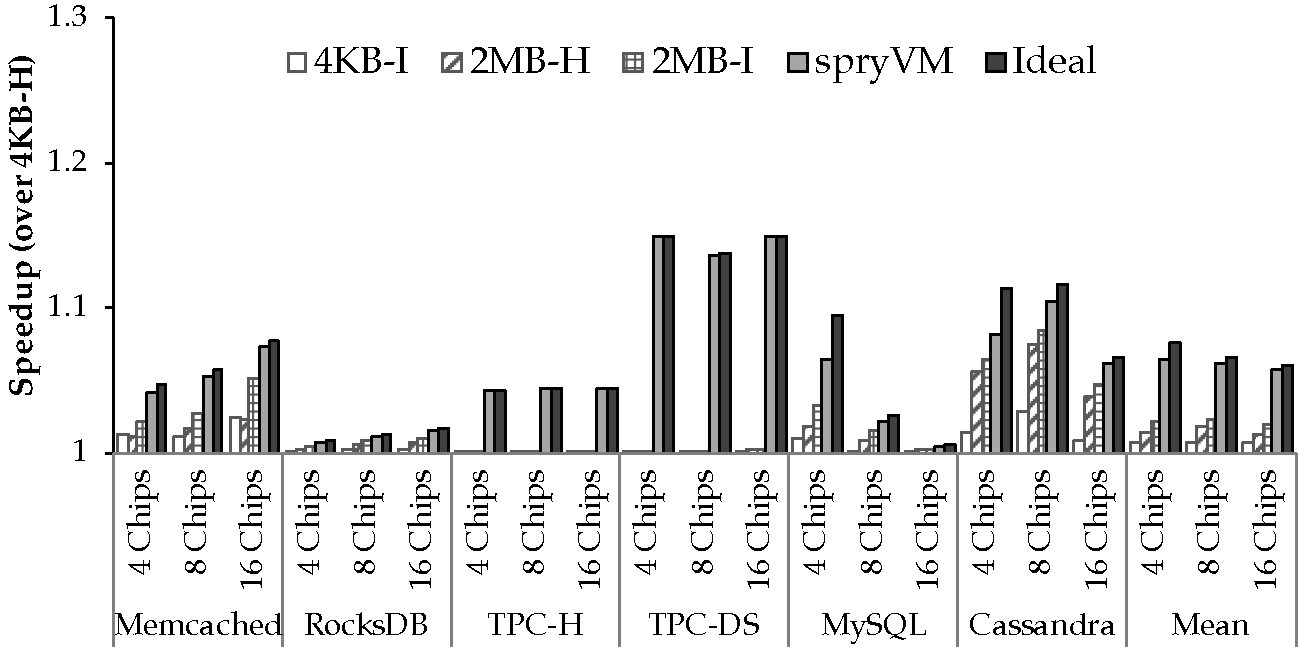
\includegraphics[width=0.48\textwidth,clip]{graphs/speedup_disk.pdf}
%  }



%\caption{Speedup over 4KB-H for 4KB-I, 2MB-H, 2MB-I, DTRIM, and an ideal translation.}
%  \label{fig:speedup_memory}
 
%\end{figure*}

%In this section, we perform a quantitative and qualitative study of the performance of different translation mechanisms.

We now perform a quantitative and qualitative study on VM.

\subsection{Performance Analysis}

The paper discusses many different workload scenarios and system configurations. As there are way too many performance points, we will show only the scenarios that have significant performance differences. First, we will show two workload scenarios, in-memory, where the memory size is equal to the working set size (i.e., the 1x ratio), and out-of-memory, where the working set size is eight times larger than the memory size (i.e., the 1/8x ratio). Second, as the performance across different process counts does not vary significantly, we are showing the average across runs. Third, the two topologies, daisy chain and mesh, behave similarly in terms performance, and hence we also present the average of both. Last, we present the results for different memory chip counts.

Fig.~\ref{fig:speedup_memory_in} shows the speedup of five translation mechanisms over the conventional MMU using 4KB pages and the hierarchical page table, labeled 4KB-H, for the in-memory scenario. The techniques are the conventional MMU using 4KB pages and the inverted page table, 2MB pages using the hierarchical and inverted page tables, DTRIM, and an ideal translation mechanism with zero translation overhead. We label the techniques as 4KB-I, 2MB-H, 2MB-I, DTRIM, and Ideal respectively. In the interest of space, we omit the results with 1GB pages, which perform better than 4KB pages but always worse than 2MB pages. The reason is that the number of entries in the MMU for 1GB pages is significantly limited, and server workloads have a large number of virtual segments which are accessed concurrently. First, we see that DTRIM clearly outperforms 4KB-H, 4KB-I, 2MB-H, and 2MB-I. In some cases by a large margin, up to $25\%$ for TPC-H. In other cases more moderately, $2.1\%$, $2\%$, $1.3\%$, and $0.5\%$ over 4KB-H, 4KB-I, 2MB-H, and 2MB-I respectively for MySQL. Most importantly, DTRIM is consistently on par with the ideal translation that incurs zero overhead for translation. Overall, DTRIM improves performance by $17.2\%$. $14\%$, $12.3\%$, and $10.5\%$ over 4KB-H, 4KB-I, 2MB-H, and 2MB-I respectively, and stays within 1.2\% of the ideal translation mechanism on average.

Fig.~\ref{fig:speedup_memory_out} presents the speedups for the out-of-memory scenario. As expected, the speedups are less significant that in the in-memory case. The reason is that all the cases incur the slowdown of resolving page faults, and therefore there are fewer accesses that can be accelerated. Still, DTRIM systematically performs better than the conventional MMU, $6.1\%$, $5.4\%$, $4.5\%$, and $4\%$ on average over 4KB-H, 4KB-I, 2MB-H, and 2MB-I respectively, and stays within 0.6\% of Ideal. 

Importantly, we model a greatly optimistic case when using $2$MB and $1$GB pages as we assume all pages are huge, with no generation overhead or fragmentation in any scenario. Additionally, we do not account for the excess in IO traffic generated by writing back dirty huge pages. Therefore, we expect further improvements with a realistic overhead. 

%Furthermore, we are conservatively assuming that all conflict page faults are major, and hence involve an access to secondary storage. Hence, in a real system, our speedups would likely be higher.


\subsection{Comparison with Other Proposals}

All the recent proposals on address translation for CPUs presented in Section~\ref{sec:uvm} aim to enhance the reach of TLBs by exploiting the contiguity available in the virtual and physical address spaces. Hence, these techniques are orthogonal to DTRIM as we reduce the TLB miss penalty. 

However, these techniques would be only effective for in-memory scenarios, and perform poorly for larger-than-memory working sets. In out-of-memory scenarios, direct segments~\cite{basu:efficient} would not be able to allocate the most frequently used pages in memory. Similarly, Redundant Memory Mappings and Hybrid TLB Coalescing~\cite{karakostas:redundant, park:hybrid} would not be able to allocate contiguous chunks of physical memory and fall back to base pages. CoLT~\cite{pham:colt} and Clustered TLBs ~\cite{pham:increasing} would also perform similar to the conventional translation when there is limited physical contiguity available. 

Even for in-memory scenarios, large address translation contiguity, on which proposed
TLB coalescing techniques rely~\cite{haria:devirtualizing,karakostas:redundant,gantz:hybrid,pham:colt,pham:increasing}, diminishes as the system runs. We adapt a representative kernel modification (increasing the max order of the buddy allocator), which enables large contiguous memory allocation (up to 1GB), to demonstrate the impact of memory fragmentation from long-run systems. We run a simple program \textit{mem\_sweep}, which allocates 30GB memory and accesses throughout all of it, along with our benchmarks back-to-back in our experimental machine with 32GB memory and measure the number of 1GB contiguous memory regions created by the modified kernel. Our program is able to obtain 28 of 1GB contiguous memory regions right after our experimental machine boots. The number decreases substantially to 8 at second round of execution and goes down to 5 (18\% of the number of 1GB contiguous memory regions at fresh boot time) after another 4 rounds of execution. The results show that memory fragmentation can significantly deter the contiguous memory creation, especially when the system's memory is fully utilized.

\section{Evaluation}
\label{sec:evalation}

In this section, we evaluate SpryVM with conventional translation using $4$KB and $2$MB pages, and qualitatively with the other prior work.   

\begin{figure*}[t]
	\centering
	\subfloat[Hash Table]{
		\label{fig:memcached_2p_assoc}
		\includegraphics[width=0.3\textwidth,clip]{graphs/HT_32GB.pdf}}
	\subfloat[Skip List]{
		\label{fig:memcached_4p_assoc}
		\includegraphics[width=0.3\textwidth,clip]{graphs/SL_32GB.pdf}}
	\hspace{.01in}
	\subfloat[BST Internal]{
		\label{fig:rocksdb_2p}
		\includegraphics[width=0.3\textwidth,clip]{graphs/BSTI_32GB.pdf}}
	\subfloat[BST External]{
		\label{fig:rocksdb_4p}
		\includegraphics[width=0.3\textwidth,clip]{graphs/BSTE_32GB.pdf}}

	
	\caption{TLB sensitivity study for 32GB working set for conventional translation with 4KB and 2MB pages and SpryVM.
		\label{fig:miss_ratio_32GB}}
\end{figure*}

\begin{figure*}[t]
	\centering
	\subfloat[Hash Table]{
		\label{fig:memcached_2p_assoc}
		\includegraphics[width=0.3\textwidth,clip]{graphs/HT_128GB.pdf}}
	\subfloat[Skip List]{
		\label{fig:memcached_4p_assoc}
		\includegraphics[width=0.3\textwidth,clip]{graphs/SL_128GB.pdf}}
	\hspace{.01in}
	\subfloat[BST Internal]{
		\label{fig:rocksdb_2p}
		\includegraphics[width=0.3\textwidth,clip]{graphs/BSTI_128GB.pdf}}
	\subfloat[BST External]{
		\label{fig:rocksdb_4p}
		\includegraphics[width=0.3\textwidth,clip]{graphs/BSTE_128GB.pdf}}
	
	
	\caption{TLB sensitivity study for 128GB working set for conventional translation with 4KB and 2MB pages and SpryVM.
		\label{fig:miss_ratio_128GB}}
\end{figure*}

\subsection{TLB Sensitivity}

~\subsubsection{32GB working set.} Figure~\ref{fig:miss_ratio_32GB} shows the TLB miss ratio as we increase the number of entries, of the four data structure traversals, hash table, skip list, binary search tree internal, and binary search tree external, with a working set size of $32$GBs. Each graph plots three lines. The blue line represents the conventional translation mechanism using 4KB pages. The orange line the same mechanism but using $2$MB pages. The gray bar represent the TLB miss ratio of SpryVM, which uses $4$KB pages.

\noindent\textbf{4KB pages:} For all four data structures, SpryVM
systematically beats conventional translation with $4$KB pages given
the same TLB size. For example, for the hash table, conventional
translation requires a 128-entry TLB to match the miss ratio of SpryVM
with 8 entries, a $16\times$ difference. Furthermore, we see that the
gap between the efficiency of TLBs worsens with the absence of data
locality. For the skip list, which is the workload with the lowest
data locality, conventional translation requires around $2048$ entries
to match the miss ratio of SpryVM with 16 entries.

\noindent\textbf{2MB pages:} Using $2$MB pages improves the TLB
behavior of conventional translation. For example, for the hash table,
with 2MB pages, conventional translation only need 8 entries to match
the miss ratio of 4 entries in SpryVM, a $2\times difference$. In
contrast, in workloads where there exist data locality, like in the
trees, in which there is data reuse for the higher levels of the tree,
the per-region $4KB$ pages are not able to beat $2$MB pages. However,
note that $2$MB are not always available (as explained in the
background section) and we could also employ $2MB$ pages for SpryVM;
we defer that approach for future work. Furthermore, in workloads
where there exists no locality, such as in the skip list data
structure, $2$MB deliver an almost negligible improvement with respect
to $4KB$ pages (also shown in prior work for other data structure with
low data locality like graphs~\cite{haria:devirtualizing}). Hence, for
the skip list, the number of TLB entries still needs to be $16\times$
bigger to match SpryVM's TLB area efficiency.

~\subsubsection{128GB working set.} Figure~\ref{fig:miss_ratio_128GB}
shows the TLB miss ratio as we increase the number of entries of the
four data structure traversals with a working set size of
$128$GBs. Similarly to the previous set of graphs, each graph plots
three lines: conventional translation with 4KB pages, the same
mechanism but using $2$MB pages, and SryVM, which uses $4$KB pages.

\noindent\textbf{4KB pages:} For all four data structures, SpryVM
systematically beats conventional translation with $4$KB pages given
the same TLB size. Furthermore, the area-efficiency gap is more
pronounced as the working set is larger.

\noindent\textbf{2MB pages:} Although $2$MB pages helps to reduce the
area-efficiency gap with respect to $4$KB and SpryVM, the increase in
the working set worses the benefits. For example, in the hash table,
$2$MB pages now requires $8\times$ the number of TLB entries to match
the miss ratio of 4 TLB entries in SpryVM. Furthermore, in the cases
where there is more data locality, the situation also worsens, and in
fact, for the binary search tree external, now $2$MB pages and SpryVM,
behave almost identically.

\subsection{TLB Miss Penalty}

SpryVM does not only improve the area-efficiency of TLBs but also reduces the TLB miss penalty. Figure~\ref{fig:penalty} shows the TLB miss penalty of a memory reference, including the data access to memory, normalized to the ideal translation mechanism where only the data access of the memory references is required. We decided to be conservative and assume perfect MMU caches, and therefore page walks requires only one memory reference. The reason is because we want to decouple the TLB miss penalty benefits from the page table implementation, since in our case, with an inverted page table of $1/4x$ of load factor, we are able to guarantee one memory reference per page walk, whereas the hierarchical four-level page table requires a very significant MMU cache hierarchy. Furthermore, we consider two systems, a conventional two-socket machine and a large-memory eight-socket machine.

As the figure shows, page walks in a conventional VM mechanism requires a memory reference to locate the page table entry, and hence a memory reference requires two memory accesses. In contrast, and as explain in Figure~\ref{fig:pagewalk_partition_miss}, the virtual address uniquely identifies the memory region, and hence the time it takes to locate the region, traversing the NoC and off-chip interconnects is overlapped with the data path. Furthermore, the larger the memory systems, the larger the contribution of the network time in the page walk time, and hence the large the reduction in page walk time with respect with conventional translation. 

\begin{figure}[t]
	\centering
	\includegraphics[width=0.8\columnwidth]{graphs/penalty.pdf}
	\caption{TLB miss penalty for conventional and SpryVM.}
	\label{fig:penalty}
\end{figure}

\subsection{Associativity study of VM}

\begin{figure*}
	\centering
	\subfloat[Memcached --- 1 Process]{
		\label{fig:memcached_1p}
		%  \includegraphics[width=.32\textwidth,clip,trim = 18mm 213mm 117mm 20mm]{figs/eps/sim-rread-lat.eps}}
		\includegraphics[width=.365\textwidth,clip]{graphs/memcached_assoc_1p-bw.pdf}}
	%  \hspace{.01in}
	\subfloat[RocksDB --- 1 Process]{
		\label{fig:rocksdb_1p}
		%  \includegraphics[width=.32\textwidth,clip,trim = 18mm 213mm 115mm 20mm]{figs/eps/sim-rread-bw.eps}}
		\includegraphics[width=.31\textwidth,clip]{graphs/rocksdb_assoc_1p-bw.pdf}}
	%   \hspace{.01in}
	\subfloat[Cassandra --- 1 Process]{
		\label{fig:cassandra_1p}
		%  \includegraphics[width=.32\textwidth,clip,trim = 28mm 217mm 115mm 20mm]{figs/eps/emu-rread-lat_cropped.eps}}
		\includegraphics[width=.31\textwidth,clip]{graphs/cassandra_assoc_1p-bw.pdf}}
	\caption{Overall miss ratio broken down into compulsory, capacity, and conflict misses.
		\label{fig:miss_ratio}}
\end{figure*}

\begin{figure*}[t]
	\centering
	\subfloat[Memcached --- 2 Processes]{
		\label{fig:memcached_2p_assoc}
		\includegraphics[width=.36\textwidth,clip]{graphs/memcached_assoc_2p-bw.pdf}}
	\subfloat[Memcached --- 4 Processes]{
		\label{fig:memcached_4p_assoc}
		\includegraphics[width=.31\textwidth,clip]{graphs/memcached_assoc_4p-bw.pdf}}
	\subfloat[Memcached --- 8 Processes]{
		\label{fig:memcached_8p}
		\includegraphics[width=.31\textwidth,clip]{graphs/memcached_assoc_8p-bw.pdf}}
	
	
	
	\caption{Overall miss ratio broken down into compulsory, capacity, and conflict misses.
		\label{fig:miss_ratio_procs}}
\end{figure*}

\subsection{Single-Process In-Memory}

Fig.~\ref{fig:miss_ratio} shows results for three single-process workloads: Memcached, RocksDB, and Cassandra. The y-axis breaks down the total misses into the three distinct miss classes. Each category on the x-axis corresponds to the ratio between the size of the physical memory and the size of the application's working set. For example,  $8\times$ indicates that the memory is eight times larger than the application's working set. Similarly, $1/2\times$ means that the application's working set is twice the size of the memory. We collapse results for $8\times$ to $1\times$ because they are similar and visually identical; each case represents a fully in-memory scenario. Furthermore, within each working set category, the x-axis sweeps through different VM associativities, from direct-mapped to 32-way associative. 



Even with a simple direct-mapped translation, compulsory misses represent $99.9\%$ of all the misses. There are no capacity misses as the working set fully fits in memory. Conflict misses are scarce. For example, Memcached using direct-mapped translation achieves a conflict miss rate in the order of one miss per $10^{8}$ memory accesses. Using $2$ ways removes all the conflicts for the $8\times$, $4\times$, and $2\times$ cases, while $4$ ways are required for the $1\times$ case (where the memory size is equal to the size of the working set). For in-memory scenarios, page conflicts arise because the virtual address space of server applications is particularly sparse; there are many virtual segments scattered all over the address space. For example, Java processes exhibit many virtual segments due to the dynamic nature of the JVM. This is best observed in the case of Cassandra, which exhibits direct-mapped conflict miss rates in the order of one miss per $10^{7}$ and $10^{6}$ memory accesses for the $8\times$--$2\times$ cases and the $1\times$ case respectively. However, conflict misses drop rapidly as associativity increases and using 4 ways removes all conflicts for the $4\times$ and $2\times$ cases, while virtually eliminating conflicts for the $1\times$ case. The observation that conflict misses drop rapidly with associativity has also been shown for caches~\cite{hill:aspects, cantin:cache}. We elide the results for TPC-H, TPC-DS, and MySQL as they follow identical trends.

\subsection{Single-Process Out-of-Memory}

In contrast to in-memory scenarios, when the working sets do not fit in memory ($1/2\times$, $1/4\times$, $1/8\times$ cases), capacity misses grow with the working set size, while the fraction of compulsory misses drops. Although conflict misses are more significant than in the in-memory scenarios, conflicts drop sharply after 2-4 ways. In the worst case, 16 ways are required to drive conflict misses down to $\sim1\%$ of all the misses. Note that Cassandra has an active working set that fits in a memory of $1/4\times$ the data size, and capacity misses start to rise at the $1/8\times$ case and beyond. Fundamentally, all these results corroborate the seminal work on caches~\cite{hill:aspects, cantin:cache}. 

\subsection{Multi-programming In-Memory}
Fig.~\ref{fig:miss_ratio_procs} presents results for multi-programming. We take each of the three workloads, Memcached, RocksDB, and Cassandra, and increase the number of processes, keeping the overall working set size the same with respect to the single process scenarios. For example, for the $1\times$ case in Fig.~\ref{fig:miss_ratio}, the working set of a single process equals the size of the memory. In Fig.~\ref{fig:miss_ratio_procs}, for two processes sharing the same physical memory, the per-process working set is half the size of the physical memory. Similarly, with four processes, per-process working sets consume a quarter of the physical memory. We thus guarantee that only the increase in the number of processes has an impact on the associativity. 

For in-memory scenarios ($8\times$--$1\times$ cases), once the associativity equals the number of processes, compulsory misses represent $99.9\%$ of all the misses for all the workloads. Increasing the associativity further makes conflicts virtually disappear after a few additional ways. For instance, for Memcached, with 8, 16, and 32 ways, the conflicts are in the order of a single miss per $10^{9}$ accesses for 2, 4, and 8 processes, respectively. Cassandra requires 4, 8, and 8 ways to achieve a miss conflict rate of one miss per $10^{9}$ accesses for 2, 4, and 8 processes, respectively. Again, the trends are identical for TPC-H, TPC-DS, and MySQL. Overall, conflict misses become virtually zero with a few ways (i.e., 2-4) per process.

\subsection{Multi-programming Out-of-Memory}

For the cases where the working sets do not fit in memory, the trends are similar to the single-process scenarios. Capacity misses become more significant as the working set sizes grow, making conflict and compulsory misses less important. Similar to the in-memory case, once the associativity equals the number of processes, the fraction of conflict misses matches the single-process results. Conflicts drop rapidly as in the other cases and with 4 ways per process, conflict misses remain within $1\%$ of the total misses for all the workloads. The results for TPC-H, TPC-DS, and MySQL are identical.

\subsection{Linux Prototype}
\begin{figure}[t]
   \centering
   \includegraphics[width=1.0\columnwidth]{graphs/realhw.pdf}
   \caption{Page fault rate vs memory size for fully associative (1-node) and set-associative (32-nodes).}
   \label{fig:realhw}
\end{figure}


We successfully ran all server workloads on modified linux with 32 memory regions (nodes), utilizing above 90\% of available DRAM without a single page fault. Figure~\ref{fig:realhw} shows the page fault rate RocksDB tuned for a 16GB footprint, as we vary the available memory capacity in the critical range using the linux boot-time mem parameter. First, we note that our kernel properly deals with demand paging in the out-of-memory scenarios. Second, we see that the page fault rates in fully associative (1 partition) and set-associative (32 partitions) case follow the same trend, except that the 32-partition setup requires about 1.5--2GB more memory to achieve the same page-fault rate. We note that this is not related to associativity, given that the associativity reduction is minor. Instead, this effect is the artifact of the prototype that relies on linux NUMA nodes, which have small memory overheads per node and exhibit a degree of variability in their capacity. 

\begin{figure}[t]
	\centering
	\subfloat[32GB]{
		\label{fig:memcached_2p_assoc}
		\includegraphics[width=0.25\textwidth,clip]{graphs/speedup_32GB.pdf}}
	\subfloat[128GB]{
		\label{fig:memcached_4p_assoc}
		\includegraphics[width=0.25\textwidth,clip]{graphs/speedup_128GB.pdf}}

	\caption{Speedup of conventional translation with $2$MB pages and SpryVM, with respect to conventional $4$KB pages.
		\label{fig:perf}}
\end{figure}

\subsection{Performance}

Figure~\ref{fig:perf} compares the performance of $2$MB pages and SpryVM, with respect to a conventional translation mechanism using $4$KB pages, for $32$GB and $128$GB cases. SpryVM clearly outperforms $4$KB pages in both working set scenarios, by up to $1.8\times$ with $32$GB and $1.7\times$ on average. Furthermore, in $128$GB scenarios, SpryVM outperforms $4$KB pages by up to $2.36\times$ and $2.18\times$ on average. Compared to conventional translation with $2$MB pages, SpryVM outperforms it by up to $1.7\times$ and $1.2\times$ on average for $32$GBs, and by up to $2.15\times$ and $1.6\times$ on average for $128$GB. Furthermore, there is no case in which $2$MB pages outperforms SpryVM in the large-memory scenario.


\section{Discussion \& Future Work}
\label{sec:discussion}

Following the prior work, we assumed that the accelerators do not have caches~\cite{haria:devirtualizing, picorel:near-memory}, as they are usually tailored for acceleration of data traversals that are not cache friendly. However, DTRIM is equally applicable to systems with caches, as well as the systems with execution-side TLBs and MMUs. In such cases, DTRIM would be very useful in accelerating the handling of TLB misses. Recent practical designs for virtual cache hierarchies~\cite{yoon:revisiting, park:efficient} would also be a great fit for DTRIM, obviating the need for execution-side TLB hardware. Also note that DTRIM could be used for accelerating CPU TLB misses, which we plan to explore in the future. 

DTRIM's memory-side translation hardware could be looked at as a fully distributed IOMMUs. The key difference is that IOMMUs serve translation/TLB miss requests for the devices attached to the local socket, but in doing so they cache translations and perform page walks across the entire memory system, while DTRIM's translations and page walks are confined within the local memory partition, which is a key to scalability. 

%\noindent\textbf{Page faults.} Upon a page fault triggered by an MPU, we choose to interrupt the CPU to run a handler, as MPUs may not be capable of running an OS. The memory-side MMU notifies the MPU of the fault, and then the MPU places a request in a memory-mapped queue indicating the faulting virtual address and MPU's id. Then, it raises an interrupt on the CPU. The handler running on the CPU resolves the page fault and updates both the CPU's and memory-side MMU's page table. All MMU state is exposed through memory-mapped IO with an uncacheable memory policy. Once the fault is serviced, the handler notifies the appropriate MMU, which resumes execution and retries the faulting address. Such page fault processing is also employed in today's integrated GPUs~\cite{vesely:observation}.\\

%\noindent\textbf{TLB shootdowns.} Many ways exist to maintain the memory-side page tables coherent upon TLB shootdowns initiated by the CPU.  Our approach is similar to those used in integrated GPUs: an OS driver monitors any changes on virtual address spaces shared with MPUs, triggering update operations for the affected page table entries. Note that the inverted nature of the page tables eliminates any global coherence activity in the memory network as a virtual page maps to only one partition, and consequently, page table. Additionally, modifying the desired page table entry requires a single memory access in the common case, accounting for at most a few hundred nanoseconds. This additional overhead is not as significant as the TLB shootdown operation itself, which removes the stale entries in the TLBs of MPUs and CPU cores, and already takes tens of microseconds~\cite{oskin:software-managed}.\\

%\mjs{does this imply that all MPU translations are snooped into the CPU? discuss scalability?}

%\noindent\textbf{Cache hierarchy.} We assume that accelerators, much like conventional cores, could integrate te physical caches and an execution-side MMU with TLBs. Upon a page walk, the memory-side MMUs reply with the page table entry and cache block, which are stored in the MMU's TLB and data cache respectively. However, to avoid TLBs and TLB shootdowns~\cite{villavieja:didi}, we could use virtual caches. Recent practical designs for virtual cache hierarchies~\cite{yoon:revisiting, park:efficient} would be a perfect fit for DTRIM. In this approach, MPUs access the cache with virtual addresses, and upon a cache miss, the request is propagated to the memory-side MMUs to translate and fetch the corresponding block. The memory-side MMU only replies with the data cache block, simplifying our design.     

%\noindent\textbf{Synonyms.} In our current design, all the synonyms of a particular page frame need to map to the same memory set or partition. We believe this is not a significant limitation as it has been already included in commercial systems~\cite{cheng:virtual}. Nevertheless, our page table entries contain the whole page frame address, and hence with a slight modification in our design, we could enable synonyms to map anywhere. The only potential consequence is a drop in performance as a synonym page might map to a page frame residing in another memory partition. However, prior work has already shown that synonyms are both scarce and infrequent~\cite{yoon:revisiting, basu:reducing, park:efficient}, and therefore this overhead should be negligible.\\

%\noindent\textbf{DIPTA for CPUs.} DIPTA is a near-memory structure independent of any control flow, and any execution unit can use it to eliminate the translation overhead for the part of memory covered by DIPTA. While the focus of this work is on MPUs, CPUs can use DIPTA the same way MPUs do. However, CPUs may have to continue using TLBs in order to efficiently address any planar DDR chips and maintain full flexibility.\\

%\noindent\textbf{Multi-level memories.} Though prior work on MPUs assumes a single level~\cite{gao:practical, ahn:scalable, pugsley:ndc, ahn:pim-enabled}, memory can be organized as a hierarchy, with a die-stacked cache~\cite{reinders:knights, volos:fat} backed up by planar memory. For hardware-managed caches, the memory-side MMU performs the translation and accesses the partition, and in case of a cache miss, the page is fetched from planar memory as part of the standard cache miss operation. Once the page arrives into the partition, the data is sent back to the MPU. Note that moving the page from planar memory to the 3D memory does not affect the page table entry. In software-managed caches~\cite{reinders:knights}, MPUs rely on a software API for explicit migration of pages into the die-stacked memories.

%, as MPUs cannot access planar memory directly. 

%\noindent\textbf{Kernel memory.} We consider user instructions only as we argue that MPUs, like all prior custom hardware (e.g., GPU, FPGA), should execute only user code. Nevertheless, DTRIM is a great fit for the kernel, as Linux and FreeBSD's memory usage is almost entirely direct-mapped~\cite{mauerer:professional, mckusick:design} and memory resident. The TLB's tag matching logic would only require to skip the ASID bits for kernel accesses.

%As all the processes share the same kernel virtual addresses, the logic needs to ignore the ASID bits for kernel accesses. The implementation is trivial as Linux and FreeBSD partition the address space into two halves.

%, and hence the virtual address dictates whether to ignore the ASID bits.

%\mjs{does this imply that you want to run the kernel in the MPUs? i'm nto sure why this is an issue for your technique if only the CPU runs the kernel, all of its translations will just stay local and the MPUs will run their user-level code happily in the distance}

%\noindent\textbf{OS support.} The OS only needs to guarantee that the virtual page number and the page frame number map to the same memory set. OSs that support virtual caches already provide this capability (e.g., Solaris~\cite{cheng:virtual} and MIPS OS~\cite{taylor:tlb}). Therefore, the required modifications to OSs that do not have this feature should be feasible.



\section{Related Work}
\label{sec:relatedwork}

%\noindent\textbf{Near-memory processing.} Advancements in die-stacking have enabled the integration of logic into DRAM chips~\cite{hmc, diram}. Leveraging this technology, several domain-specific architectures have emerged. NDC~\cite{pugsley:ndc}, Tesseract~\cite{ahn:scalable}, and NDP~\cite{gao:practical} consider a network of MPU chips with low-power cores. Neurocube~\cite{kim:neurocube} proposes the usage of programmable custom logic to accelerate neural networks. A few works aim to exploit 3D memories for database operators~\cite{xi:beyond,mirzadeh:sort, power:implications, drumond:mondrian}. 

%Unified VM is either supported with conventional address translation~\cite{pugsley:ndc, gao:practical} or deferring translation to the CPU cores or IOMMUs~\cite{xi:beyond}.

%namely the scan operator with GPUs~\cite{power:implications} and custom logic~\cite{xi:beyond}, and the join operator with microcontrollers~\cite{mirzadeh:sort}. 

%Integrating DRAM and computation has been an active area of research for decades. In the early 90s, IRAM~\cite{kozyrakis:scalable} advocated for dedicating the on-chip transistors to DRAM in future billion-transistor chips. Active Pages~\cite{oskin:active} proposed a protocol to orchestrate the execution of code on reconfigurable logic next DRAM. FlexRAM~\cite{kang:flexram} and DIVA~\cite{draper:architecture} considered an array of microcontrollers next to DRAM, controlled by the host CPU. However, the ever-growing demands for more memory capacity, along with the density gap between smart memories and DRAM-only memory chips hampered their adoption. 

%A couple of works aim to exploit the abundant internal bandwidth to database operators. The scan operator, with GPUs and CITE with custom logic, and the join operation, with a micro-controller. 

%Tesseract relies on MPI without virtual memory. NDC and NDP assume a global address space with conventional address translation. Ahn et al.~\cite{ahn:pim-enabled} execute some ISA instructions of the host next to the memory, while translation is performed on the CPU.\\

%\noindent\textbf{Unified virtual memory} Industry and academia have been recently pushing towards a unified virtual memory between CPUs and GPUs. Industry examples include the HSA Foundation~\cite{hsa} and Nvidia's Unified Memory~\cite{harris:unified}. Academic publications~\cite{power:supporting, pichai:architectural} propose a TLB architecture to sustain the high translation throughput required for GPU cores. A recent study on IOMMU translation for integrated GPUs has shown that a TLB miss takes an order of magnitude longer than on CPU cores~\cite{vesely:observation}. 

%Several studies exploited the contiguity generated by using the buddy allocator and memory compactor to increase the TLB reach. 

%CoLT \cite{pham:colt}, Clustered TLBs\cite{pham:increasing}, and sub-blocked TLBs\cite{talluri:surpassing} group multiple PTEs into a single TLB entry. Direct segments~\cite{basu:efficient} allows for an efficient mapping between a single virtual segment mapped contiguously in physical memory. Karakostas et al.~\cite{karakostas:redundant} propose a fully associative range-based TLB and page table to transparently exploit the available contiguity in the physical memory. Transparent Huge Pages~\cite{transparenthugepages} and libHugeTLBFS~\cite{lighugetlbfs} increase the TLB reach by mapping large regions to a single TLB entry.

\noindent\textbf{Improving TLB performance.} The techniques of Section~\ref{sec:uvm} improve the TLB reach. In contrast, other techniques target reducing the TLB miss penalty. Commercial processors store page table entries in data caches to accelerate page walks~\cite{intel:architectures}. Some architectures use page table caches (e.g., TSBs in SPARC~\cite{sun:ultrasparc}). MMU caches are employed to skip walking intermediate page table levels~\cite{bhattacharjee:large-reach, barr:translation}. Other techniques translate speculatively~\cite{barr:spectlb} or prefetch TLB entries~\cite{bhattacharjee:characterizing}. 

%~\cite{pham:colt, pham:increasing, basu:efficient, karakostas:redundant, transparenthugepages, lighugetlbfs, park:hybrid}

\noindent\textbf{Reducing VM associativity.} We are not the first to restrict VM associativity. Several degrees of page coloring---fixing a few bits from the virtual-to-physical map---were proposed in the past. The MIPS R6000 used page coloring coupled with a small TLB to index the cache under tight latency constraints~\cite{taylor:tlb}. Page coloring has also been used for virtually indexed physically tagged caches~\cite{chiueh:eliminating} as an alternative to large associativities~\cite{gustafson:ibm} or page sizes~\cite{jouppi:architectural}. Alan Jay Smith~\cite{smith:comparative} advocated the usage of set-associative mappings for main memory to simplify page placement and replacement. 

%---much like another cache level---to 

%\javier{Should I remove from the above how translation is performed? Then I talk about it below.} \\
%\javier{Talk about DNNs on 3D memories}\\
%\javier{Add HPCA paper on virtual memory for accelerators} \\
%\javier{Rewrite it to talk about unified virtual memory.}\\

%\noindent\textbf{Page Tables.} Hierarchical, linear, inverted. Software caches for page tables. \javier{Talk about page table caches (e.g., TSB)}\\


\section{Conclusion}
\label{sec:conclusion}

In this work, we show that the full associativity of VM is largely unnecessary, as the majority of misses are either compulsory or capacity, and hence insensitive to associativity. By restricting the associativity to identify a memory chip and partition uniquely, memory can be accessed as soon as the virtual address is known, while a memory-side TLB translates and fetches the data, overlapping both operations almost entirely. By implementing this concept in stock Linux prototype, we show that set-associative memory can be easily implemented using the existing Linux code paths. 


%we perform an associativity study of VM across a variety of scenarios and conclude that capacity and compulsory misses dominate the overall misses, while conflict misses, which associativity alleviates, rapidly drop as the VM associativity increases. Hence, the full associativity of VM remains largely unused. 

%Dramatic advances in 3D integrated circuits have enabled the integration of memory and logic in the same chip. 

\newpage




\bibliographystyle{plain}
\bibliography{references}
%\bibliographystyle{IEEEtranS}
%\bibliography{refs}


\end{document}

